\documentclass{article}
\usepackage{graphicx,xcolor}
\usepackage{fancyvrb}
\usepackage[colorlinks=true,urlcolor=blue,linkcolor=cyan]{hyperref}
\usepackage{sidenotes}
\usepackage[toc]{glossaries}
\newglossary[nlg]{variable}{vin}{vot}{List of variables}
\newglossary[nlg]{parameter}{pin}{pot}{List of Aggregate Parameters}
\newglossary[nlg]{parameter1}{p1in}{p1ot}{List of individual Parameters}
\makeglossaries
%\newcommand{\doclocation}{file:///Users/giulioni/Documents/workspace/gabriele/docs}


\begin{document}

\begin{titlepage}

%	\includegraphics[width=0.15\textwidth]{example-image-1x1}\par\vspace{1cm}
	\begin{center}
	{\color{blue}\scshape\Huge CMS \par}
	\end{center}

	\vspace{2cm}

	\noindent
	{\color{blue}\scshape\Huge C}{\scshape\LARGE ommodities} 
	{\color{blue}\scshape\Huge M}{\scshape\LARGE arkets} 
	{\color{blue}\scshape\Huge S}{\scshape\LARGE imulator}\\

 
	
	\vspace{1.5cm}
	\noindent
	{\scshape\Huge Users Manual \par}

	\vspace{2cm}
	\noindent
	{\Large\itshape Gianfranco Giulioni\par}
	\vfill

% Bottom of the page
	{\large \today\par}
\end{titlepage}

\newpage
\thispagestyle{empty}

\null

\pagenumbering{roman}

\tableofcontents
 

\newpage

\newglossaryentry{var:q_moved}% label 
{% 
  type=variable,% glossary type 
  name={$q_{p^+_{\max} -> p^+_{\max}}$},% 
  description={Quantity moved from most expensive to the cheapest market session} 
}
\newglossaryentry{var:C^min_b}% label 
{% 
  type=variable,% glossary type 
  name={$C^{min}_b$},% 
  description={Consumption level of buyer $b$ below which people manage to buy more product} 
}
\newglossaryentry{var:I^d_b}% label 
{% 
  type=variable,% glossary type 
  name={$I^d_b$},% 
  description={Desired Inventories of buyer $b$} 
}
\newglossaryentry{var:I_{b,t}}% label 
{% 
  type=variable,% glossary type 
  name={$I_{b,t}$},% 
  description={Inventories of buyer $b$ at beginning of period $t$} 
}
\newglossaryentry{var:B_{b,t}}% label 
{% 
  type=variable,% glossary type 
  name={$B_{b,t}$},% 
  description={Quantity of resources bought by buyer $b$ in period $t$} 
}
\newglossaryentry{var:C_{b,t}}% label 
{% 
  type=variable,% glossary type 
  name={$C_{b,t}$},% 
  description={Consumption of resources by buyer $b$ in period $t$} 
}
\newglossaryentry{var:bar{D}_{b,ms,t}}% label 
{% 
  type=variable,% glossary type 
  name={$\bar{D}_{b,ms,t}$},% 
  description={Intercept of the $ms$ market session demand curve of buyer $b$ in period $t$} 
}
\newglossaryentry{var:ms_{b,t}}% label 
{% 
  type=variable,% glossary type 
  name={$\#ms_{b,t}$},% 
  description={number of market session buyer $b$ can participate in time step $t$} 
}
\newglossaryentry{var:Y_{p}}% label 
{% 
  type=variable,% glossary type 
  name={$Y_{p}$},% 
  description={production realized by producer $p$} 
}
\newglossaryentry{var:Y_{b,0}}% label 
{% 
  type=variable,% glossary type 
  name={$Y_{b,0}$},% 
  description={producer's $p$ average production} 
}



\newglossaryentry{par:P0}{
  type=parameter,% glossary type 
  name={$P_0$},% 
  description={Global production at initialization}
}
\newglossaryentry{par:tau}{
  type=parameter,% glossary type 
  name={$\tau$},% 
  description={Production cycle length}
}
\newglossaryentry{par:iota}{
  type=parameter,% glossary type 
  name={$\iota$},% 
  description={Share of desired consumption to compute desired inventories}
}
\newglossaryentry{par:y}{
  type=parameter,% glossary type 
  name={$y$},% 
  description={boundary of the production percentage change}
}
\newglossaryentry{par:tau_{exp}}{
  type=parameter,% glossary type 
  name={$\tau_{exp}$},% 
  description={producers interval in deciding export policy}
}
\newglossaryentry{par:tau_{imp}}{
  type=parameter,% glossary type 
  name={$\tau_{imp}$},% 
  description={buyers interval in deciding import policy}
}
\newglossaryentry{par:pr_{imp}}{
  type=parameter,% glossary type 
  name={$pr_{imp}$},% 
  description={probability that a buyer allow import when the import policy is updated}
}
\newglossaryentry{par:pr_{exp}}{
  type=parameter,% glossary type 
  name={$pr_{exp}$},% 
  description={probability that a producer allow export when the export policy is updated}
}


\newglossaryentry{par:s}{
  type=parameter1,% glossary type 
  name={$s_{b,0}$},% 
  description={Buyer's $b$ market share at initialization}
}
\newglossaryentry{par:s_p}{
  type=parameter1,% glossary type 
  name={$s_{p,0}$},% 
  description={Producer's $p$ share of global production at initialization}
}
\newglossaryentry{par:d_{b}}{
  type=parameter1,% glossary type 
  name={$d_{b}$},% 
  description={Buyer's $b$ slope of the demand curves}
}
\newglossaryentry{par:barDb0}{
  type=parameter1,% glossary type 
  name={$\bar{D}_{b,0}$},% 
  description={Intercept of buyer $b$ the demand curves in the first simulation time step}
}



%A \gls{not:set} is a collection of objects.

\printglossaries

\newpage

\pagenumbering{arabic}
\section{Overview}

The CMS has three types of agents: producers, buyers and markets.
These agents' common feature is that each of them has a geographic location given by a latitude and a longitude. 
%Producers and buyers has an additional feature: their zone. This allows us to group producers and sellers into zones. 
In the most straightforward interpretation, Producers can be thought of as sovereign countries, but it is possible to setup the model thinking at different geographical scales such as continents, macro areas, or regions of a country. For convenience of exposition we will identify hereafter producers with countries.

The model is fully customizable, however, we start describing a common setup for exposition convenience. The setup is as follows:
\begin{itemize}
	\item a produces has at least one associated buyer; in other words if a country produces it also uses the resource; 
	\item a buyer is not necessarily associated to a producer; in other words the resource can be used by countries that does not produce it;
	\item the number of markets and their geographic location is independent from the number and location of producers and buyers.
\end{itemize}
Because we think the first two listed features straightforward, we will now focus on the third one.
\subsection{Market organization}
Considering nowadays information and communication technologies, we model markets as (virtual) places where producers and buyers send information. More trivially, resources are not physically moved to the market by the producer and, once sold, moved again from the market to the buyer. As it commonly happens, buyers and sellers send their will to the market. The market uses this information to reach an agreements. Once an agreement is reached, the resources are directly moved from the seller to the buyer place.

In this context, markets geographic location does not affect producers and sellers behavior. It has a role only when the model has more than one market: opening order is set according to their latitude.

Market are organized in sessions. Each market session is associated to a producer. A producer can have only one session in a market, and must participate in at least one market. This organization allows buyers who bid in a given session to know who is the producer. The producer geographic location has an important role here because it informs buyers on where the resource is stored. Because we assume buyers bear the transport costs, the proposed markets organization allows buyers to compute such costs and account for them when submitting their bids.
\subsection{Market Participants}
A producer can always decide to sell exclusively to its associated buyer. In the real world this happen when a country forbid export. Similarly, buyers who have an associated producers can decide to buy exclusively from their producer (a producer country can forbid import). The latter, is not possible if the considered buyer has not an associated producer (a non producer country does not forbid import). 
Summing up, in each market session participates 
\begin{itemize}
	\item the producers associated with the section;
	\item buyers associated with the producer;
	\item buyers not associated with the producer if the two following condition are both satisfied:
		\begin{itemize}
			\item the producer allows export;
			\item the buyer allows import
		\end{itemize}
\end{itemize}

\subsection{Dynamics}

The ``cornerstone'' of the dynamics is the simulation time step. In each simulation time step, several action can happen, however, what mostly characterizes it is that all the market sessions are performed.  
This provides a link between real and simulated time: if we want to simulate a real world situation where markets operate once a day (week, month and so on), a simulation time step represents a day (a week, a month and so on). Staring from this observation we can comment on the other simulation events. 
Consider for example the dynamics of the resource inventories. Straightforwardly, at each time step, each buyer's inventories are increased by the quantity bought in all the market sessions it participates, while each producer's inventories are decreased by the amount sold in the market sessions it is associated. Knowing the time scale is important to model the opposite flow. For buyers, the opposite flow to purchases is consumption. Therefore, if a simulation step represents a day, we have to take into account the daily consumption. Modeling the opposite flow, is more tricky for agriculture producers. The opposite flow to sales is the production flow. Agriculture products have not a continuous production, so we cannot compute a daily, weekly or monthly produced quantity as we can do for crude oil for example. Agriculture production is in general harvested once a year. Our simulator account for this: it gives the possibility to adapt the frequency of the production flow to the model time scale. Consider for example a situation where a time step represents a month and the production cycle is a year. In this case, during the setup phase the researcher can (and must) choose to increase inventories by the obtained production every 12 simulated time steps.   

We report hereafter the sequence of events that can happen in a simulation time step. It integrates and organizes the elements given above: 

\begin{enumerate}
	\item producers decide if allow/forbid export
	\item buyers with an associated producer decide if allow/forbid import
	\item buyers update buying strategy
	\item perform market sessions
		\begin{itemize}
			\item market 1
				\begin{itemize}
				\item session 1 
					\begin{itemize}
						\item producer sends supply curve
						\item buyers send demand curves
						\item demand curves are aggregated 
						\item market price and quantity are determined
						\item buyers increase inventories by the quantity bought in this session
						\item producer decrease inventories by the quantity sold in this session
					\end{itemize}
				\item all the other sessions (if exist, perform same actions listed for session 1)
				\end{itemize}
			\item  all other markets (if exist, perform same actions listed for market 1)
		\end{itemize}
	\item buyers account consumption
	\item producers produce
\end{enumerate}

Following this list, we will now detail the simulation loop. 

\section{The loop}

\subsection{Producers decide if allow/forbid export}

Each producer has a boolean variable named \verb+exportAllowed+. 

This event consists in updating this variable with a true/false value.

At the present state, this is updated randomly. The probability that import is allowed (\gls{par:pr_{imp}}) is a parameter of the model. The researcher has to modify the \verb+stepExportAllowedFlag()+ method of the \verb+Producer+ class to model producers' export behavior.

The update frequency (\gls{par:tau_{exp}}) can be changed setting the \verb+exportPolicyDecisionInterval+ parameter as explained in section \ref{sec:parameters}.

\subsection{Buyers with an associated producer decide if allow/forbid import}

Each buyer has a boolean variable named \verb+importAllowed+. 

This event consists in updating this variable with a true/false value.

At the present state, this is updated randomly. The probability that import is allowed (\gls{par:pr_{exp}}) is a parameter of the model. The researcher has to modify the \verb+stepImportAllowedFlag()+ method of the \verb+Buyer+ class to model buyers' export behavior.

The update frequency (\gls{par:tau_{imp}}) can be changed setting the \verb+exportPolicyDecisionInterval+ parameter as explained in section \ref{sec:parameters}.

\iffalse
\vskip5mm
\noindent
updated every\\
method\\
improvement
\fi


\subsection{Buyers update buying strategy}\label{subsec:buyingStrategy}
The buying strategy is updated each simulation time step.

Updating the buying strategy is an elaborate action. It is especially because buyers have to fulfill their needs looking for cheapest opportunities in a changing environment. The most relevant change in buyers' environment is represented by the possible switch in producers export policy. In fact, buyers cannot continue buying in sessions associated to those producers who change their policy forbidding export. In these cases, buyers attempt to gather the quantities bought in these sessions in other sessions. On the other hand, new opportunities open when producers switch their policy allowing export. 

In the present version of the model, the following factors are managed during the buying strategy update:
\begin{enumerate}
	\item reducing the unit cost;
	\item allocating quantity bought in market sessions that are now not available;
	\item formulating demand in market sessions that are now available;
	\item obtaining the desired quantity.
\end{enumerate}

To understand how these tasks are implemented we specify that at each time step, each buyer send to the available sessions a demand curve.
In the current version of the model demand curves are assumed to be linear. The slope (\gls{par:d_{b}}) can be different for each buyer (see section \ref{sec:initialization}), but it is the same for the same buyer in the various market sessions. The buyer updates the buying strategy by managing the intercepts of the demand curves s/he will send to the various market sessions (\gls{var:bar{D}_{b,ms,t}}). The initial level of the demand intercepts is a parameter (\gls{par:barDb0}) (see section \ref{sec:initialization}). Summarizing, the demand in market session $ms$ formulated by buyer $b$ at time $t$ is:
\[
	D_{b,ms,t}=\bar{D}_{b,ms,t}-d_bp_{mc}
\]

Consider the following example where a buyer participated in three market sessions (labeled $A$, $B$ and $C$) in the previous period.

\vskip5mm
\hskip-1.5cm
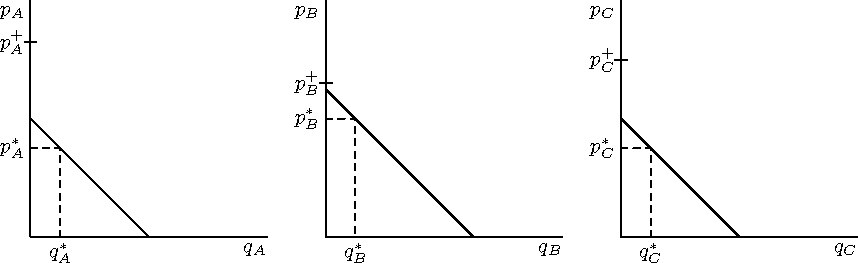
\includegraphics{fig_buying_strategy-0.pdf}

\vskip5mm
The charts show that the market prices were $p^*_B>p^*_A=p^*_C$ and that the buyer bought the quantities $q^*_A$, $q^*_B$, $q^*_C$ and the total quantity. 


% a total quantity $B_t=q^*_A+q^*_B+q^*_C$. 
Consider however, that the transport cost ($c$) must be added to the market price ($p^*$) to obtain the unit cost of the commodity. It is this cost, that we denote with $p^+$, that is used by the buyer to rank market sessions.   
Suppose now that the buyer we are considering and the producer selling in market session $C$ are from different countries and the latter forbids exports. So, the buyer have to gather the quantity $q^*_C$ in other available market sessions. The assumption is that the buyer performs this attempt in the market session with the lowest $p^+$. Looking at the chart above, we see that $p^+_B<p^+_A$. So, the demand curve in market session $B$ is shifted to the left by $q^*_C$ as happens in the following chats.   

\vskip5mm
\hskip-1.5cm
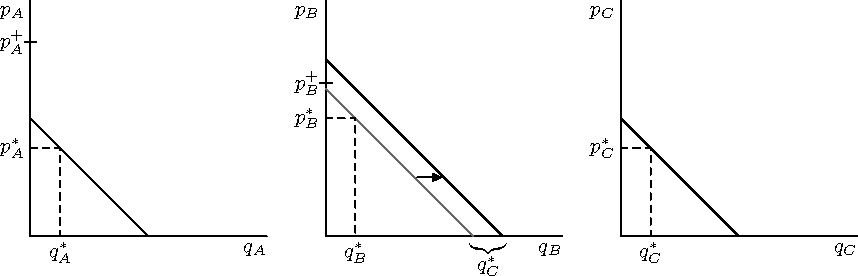
\includegraphics{fig_buying_strategy-1.pdf}

\vskip5mm
 This account for factors 1 and 2 listed above. 
However, there will be no movements in the demand curves if the buyer can continue participating in all markets sessions. The attempt to reduce the unit cost (factor 1 in the list) is lost in this case. To allow for factor 1 even when there are no export/import policy changes, we introduce the following device. The buyer moves demand from the most expensive market session ($A$ in our example) to the cheapest one ($B$). The two charts below shows the leftward shift of the demand curve in market session $A$ and the rightward shift of the curve in market session $B$.     

\vskip5mm
\hskip-1.5cm
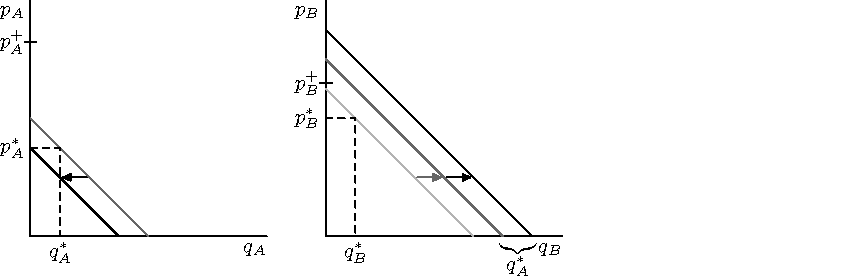
\includegraphics{fig_buying_strategy-2.pdf}
\vskip5mm

Next, consider the case in which the buyer can participate in a new market session named $D$. The problem now is how to formulate the demand curve for this new session (item 3 in the list of factors a buyer account for). The idea is that the buyer is willing to buy in this new market only if the unit cost will be lower than the lowest unit cost observed in the previous period. This allows to set the demand curve in the new market session as in the rightmost chart of the following figure. 
\vskip5mm
\hskip-1.5cm
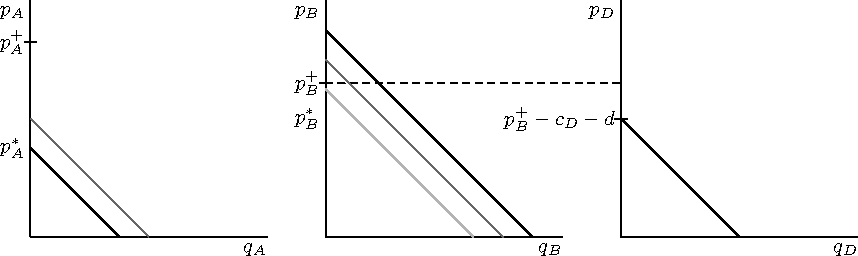
\includegraphics{fig_buying_strategy-3.pdf}


\vskip5mm
The last movement of the demand curves before sending them to the market sessions is done considering the gap between the desired level of inventories and the level of inventories under the assumption that the desired consumption could be achieved (item 4 in the list of factors a buyer account for). The mechanism is described hereafter.

The reasoning starts from the definition of Buyers' desired consumption (\gls{var:C^d_b}). It  is set at the beginning of the simulation as follows 
\[C^d_b=\frac{s_{b,0}P_0}{\tau}\]
where \gls{par:s} is the buyer market share, \gls{par:P0} is the global production at initialization, and \gls{par:tau} is the production cycle length. 
The division by $\tau$ deserves a comment. While the buying strategy is updated each simulation time step, the global production relates to the production cycle length, this motivates the division by $\tau$. An example could help clarify. Consider a situation where a simulation time step represents a month and the production is realized yearly. $P_0$ is the yearly global production and $s_{b,0}P_0$ is the amount bought yearly by the buyer. Since this event manages the monthly demand, we have to divide by 12 (which is the $\tau$ in this example.   

Buyers also has a desired level of inventories (\gls{var:I^d_b}), which is a fraction \gls{par:iota} of desired consumption
\[I^d_b=C^d_b\iota\]

At a given simulation step, a buyer starts with a level of inventory \gls{var:I_{b,t}}.

%At this point the buying strategy is updated (more below).

Consider now %, that with the updated buying strategy, 
the buyer buys an amount \gls{var:B_{b,t}} in the considered time step.

Now, it is possible to compute buyers effective consumption (\gls{var:C_{b,t}}).

If $I_{b,t}+B_{b,t}\ge C^d_b$, then $C_{b,t}=C^d_b$; otherwise  $C_{b,t}=I_{b,t}+B_{b,t}$.

The buyer enters the new period with an inventory level equal to
\[
I_{b,t+1}=I_{b,t}+B_{b,t}-C_{b,t}
\]

Note, that the buyer can also compute the quantity 
\[
	\tilde{I}_{b,t+1}=I_{b,t}+B_{b,t}-C^d_{b,t}
\]

All the demand curves are shifted by $\frac{I^d_{b}-\tilde{I}_{b,t+1}}{\#ms_{b,t+1}}$, where \gls{var:ms_{b,t}}$_{+1}$ denotes the number of market session the buyer will participate.

The following charts display the case in which the demanded quantities are increased because the level of observed inventories is lower than those desired. In fact, all the demand curve have a rightward shift. 
\vskip5mm
\hskip-1.5cm
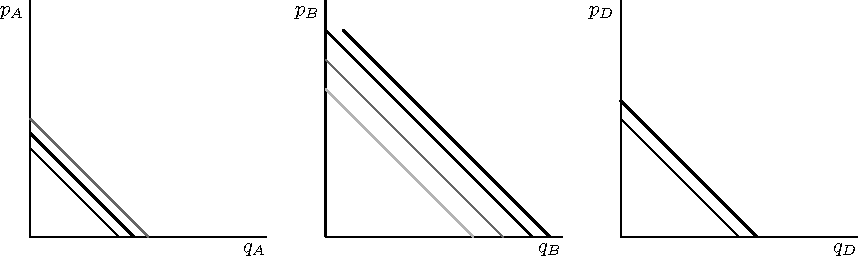
\includegraphics{fig_buying_strategy-4.pdf}

\vskip5mm
Demand curves shifts are opposite when inventories exceed the desired level.

Because there are Buyers without an associated producer, it may happen that there are no available session because all producers forbid exports. In these cases, if none of the producers switch the export policy, no demand curve is set, otherwise demand curves for newly available sessions are set. The idea is similar to that presented above, however, the buyer has not the benchmark of the cheapest unit cost at which s/he bought in the latest time step. However, the latest prices observed in the newly available market sessions are known. The current version of the model first sets the demand curve in each market in such a way that the demanded quantity is zero at the latest observed market price as displayed in the following charts. 

\vskip5mm
\hskip-1.5cm
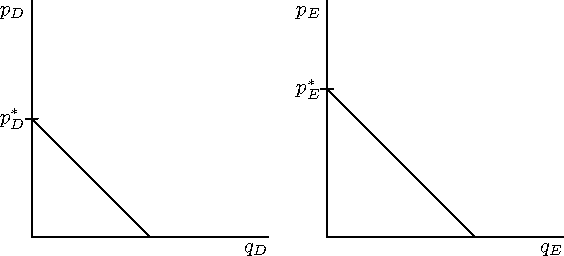
\includegraphics{fig_buying_strategy-5.pdf}

\vskip5mm
Then, the demand functions are moved as explained above according to the $\frac{I^d_{b}-\tilde{I}_{b,t+1}}{\#ms_{b,t+1}}$ quantity.

Changes to the basic behaviors presented in this paragraph can be done modifying the method \verb+stepBuyingStrategy+ of the \verb+Buyer+ class.

\subsection{Perform market sessions}

We will now describe the functioning of a market session. The program will perform the following actions for all the market sessions.

First of all, we recall that in a market session, the exchanged items come from a given producer. This is basically because using the producer's geographic location, buyers can compute transport costs that are used to update the buying strategy as explained above.

We have already discussed how buyers set their demand curves, now we need to specify how the producer sets the supply curve. In the present version of the model, the easiest option of a vertical supply curve is adopted. In other words, the supplied quantity is independent of price. Despite this simplification, managing the supply policy is tricky when accounting for production that are not realized at every simulation time step and/or for producers who participates in more than one market session in each time step. 
%In these cases, the producer has share the hold quantity among the market sessions.  
Even in these cases, the simplest solution is adopted. At the beginning of each market session, the producer checks the level of the resource stock and divides it equally among the market sessions to come before the production is realized.   

Because in a market session there is one seller (producer), its supply curve represents the whole session supply curve. Differently, we can have more than one buyer attending a session (this is usually the case except when the seller forbids exports). When we have two or more buyers, the demand curves they send to the market are aggregated by summing them horizontally to obtain the session demand curve.

Now, using the session demand and supply curves, the market price and exchanged quantity are computed. The quantity bought by each buyer is obtained using the market price and the individual demand.
The following chart, which focuses on market session $A$, can help understand.

\vskip5mm
\centerline{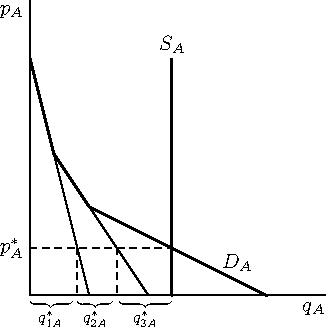
\includegraphics{fig_market_equilibrium-0.pdf}}

\vskip5mm
Bold lines are the market session supply ($S_A$) and demand ($D_A$) curves. For exposition convenience it is assumed that there are three buyers in this market. The thin black lines keep track of the horizontal sum of the individual demand curves. The intersection point between the session demand and supply curves (bold lines) determine the market price ($p^*_A$) and the total exchanged quantity ($q^*_A$). The quantity bought by each buyer ($q^*_{1A}$, $q^*_{2A}$, $q^*_{3A}$) are also reported. Obviously $q^*_A=q^*_{1A}+q^*_{2A}+q^*_{3A}$.

At the end of the session agents update their inventories level.
For buyers we have:
\[ I_b=I_b+q_{bA}\]
while for the producer
\[ I_p=I_p-q^*_A\]

This updating is performed at the end of each market session, so, in a time step, the level of inventories is updated by each agent as many time as the number of session it participates.

It can be useful to highlight the link with the notation used in section \ref{subsec:buyingStrategy}: $B_{b,t}$ is the sum of all the quantity bought by buyer $b$ in all the market sessions it participates in a given time step.   


\subsection{Buyers account consumption}

This action is performed to account for the consumption of resources occurred during the time step. Buyers' inventories are newly updated:
\[
I_b=I_b-C_b
\]
Being consumption a continuous phenomenon, this update is performed every time step.


\subsection{Producer Produce}

This action is performed to account for the production of resources. Producers' inventories are newly updated:
\[
I_p=I_p+Y_p
\]
where \gls{var:Y_{p}} is the production realized in a period. In the present version of the model it is modeled as a white noise:
\[
	Y_p=Y_{b,0}(1+u)
\]
where \gls{var:Y_{b,0}} is seller's $b$ average production computed as \gls{par:s_p}\gls{par:P0},  
and $u$ is the realization of a uniform random variable: $u\sim U(-\textnormal{\gls{par:y}},\textnormal{\gls{par:y}})$.

Differently from buyers, this update is not necessarily performed at each time step.
As mentioned above, there are commodities whose production is not continuous. For those commodities, if the time step represents a shorter time interval than the production one, this update is performed at regular interval.


\section{Installation}

In this section we describe the standard installation process needed to prepare the system to run simulations. After taking the steps described below, the user should be able to run the model regardless of the operative system s/he is using.

The model needs Repast Symphony (RS), who in turn needs the Java Development Kit (JDK). Therefore we need first to check if the JDK is installed in the system and install it if needed. Once JDK is properly running, we have to install RS. Finally the model can be installed and run in RS.

\subsection{Java Development Kit (JDK)}

Check the list of installed software to know if JDK is installed in your system. If yes, note the JDK version.
Alternatively, you can open the command line interface of your system, type \verb+javac -version+ and hit the return key. 

Once verified if JDK is installed and, if yes, its version, visit the following URL:\\
\url{http://www.oracle.com/technetwork/java/javase/downloads/index.html}\\
to know which is latest released version of JDK.

If JDK is not installed in your system or if it is not at the latest release, follow the instruction found in the JDK download page to install or upgrade it. You can also search the internet for alternative ways to install or upgrade the JDK on your system.

This installation phase is complete when the \verb+javac -version+ command returns what you expect.
If not, you should fist check if the folder containing the JDK executables are in your execution path and add it manually if needed.
Furthermore, some Linux distribution must be informed on which JDK to use using the \verb+update-alternatives+ command. 

\subsection{Repast Simphony (RS)}

The Repast suite website: \url{http://repast.sourceforge.net} has all the information needed to download and install RS.

Note that RS is provided as a plugin of the eclipse Integrated Development Environment. The Repast development team provides a customized version of eclipse, so you could encounter problems with already installed versions of eclipse. 
%Note that the streamlined installation provided below show how to avoid using eclipse.

\subsection{CMS}

CMS has to be installed as an eclipse RS project. We will give hereafter the instructions to achieve this goal.

First of all, open the eclipse downloaded and installed as described in the previous section.

Suppose your workspace has the following path:\\
\verb+/Users/coolcoder/Documents/workspace+

Open the RS perspective (window $\rightarrow$ open perspective).

Create a new RS project called \verb+cms+ (file $\rightarrow$ new $\rightarrow$ Repast Simphony project)

This creates the \verb+cms+ folder and a series of sub folders inside the workspace:

The following figure show the cms rs project folders tree.

\vskip2mm
\noindent
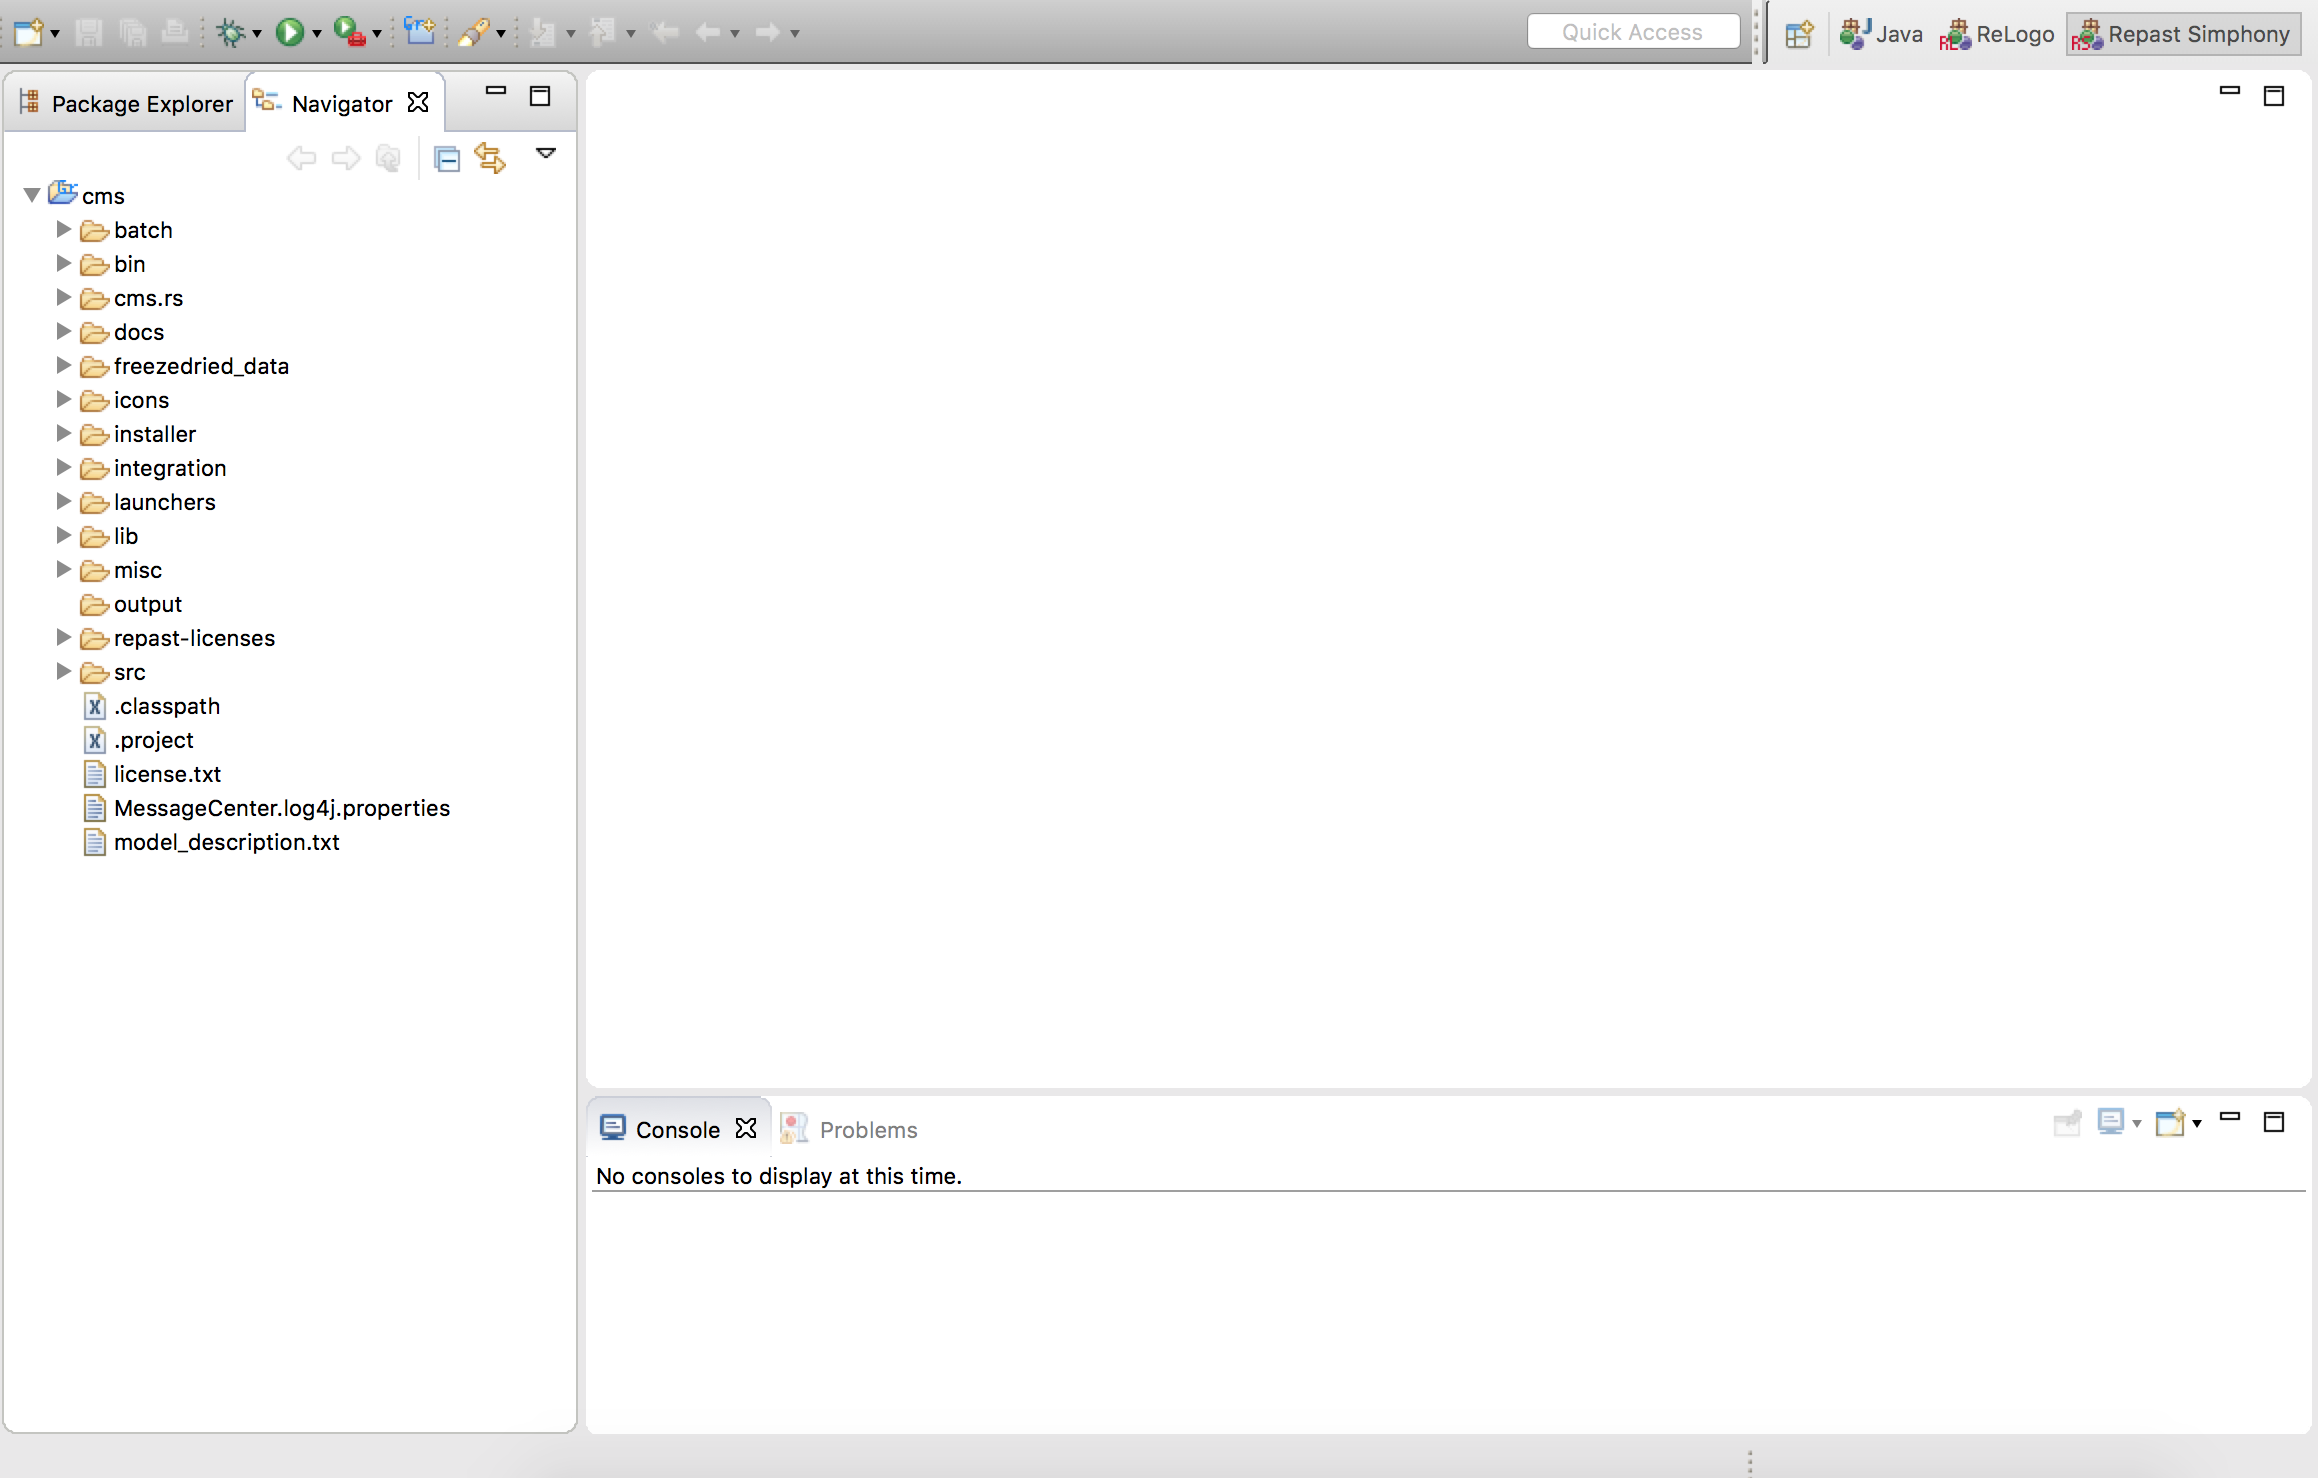
\includegraphics[scale=0.35]{fig_cms_rs_navigation}

\vskip2mm
Now, the \verb+cms+ files have to be added to the just created RS project folders tree.

We give here two alternatives: via git and using a zipped archive.

\subsubsection{Using git}

As you probably know, this is a largely used way to share the code developments.

So, let us show how to fetch the \verb+csm+ files via git. To do that, you must have a git client installed in your system. Many system comes with a git client already installed, otherwise you have to install it. Mac and windows users can consider to install the GitHub Desktop software.

You can verify if git is installed in your system by checking if your command line interface recognize the \verb+git+ command.  
If your check is successful, change directory to the \verb+cms+ project folder:\\
\verb+cd /Users/coolcoder/Documents/workspace/cms+\\
and type the following commands:
\begin{verbatim}
git init
git remote add origin https://github.com/ggiulion/cms.git
git fetch origin master
git reset --hard FETCH_HEAD
\end{verbatim}

Then, if you plan to pull or push updates, add the command:\\
\verb+git push --set-upstream origin master+

Now, the \verb+cms+ files should show up in the RS project folders.
Refresh the \verb+cms+ RS project with the navigation tab selected in the side bar (file $\rightarrow$ refresh) to make them visible in eclipse.

The following figure show how the src sub folders should look like.

\vskip2mm
\noindent
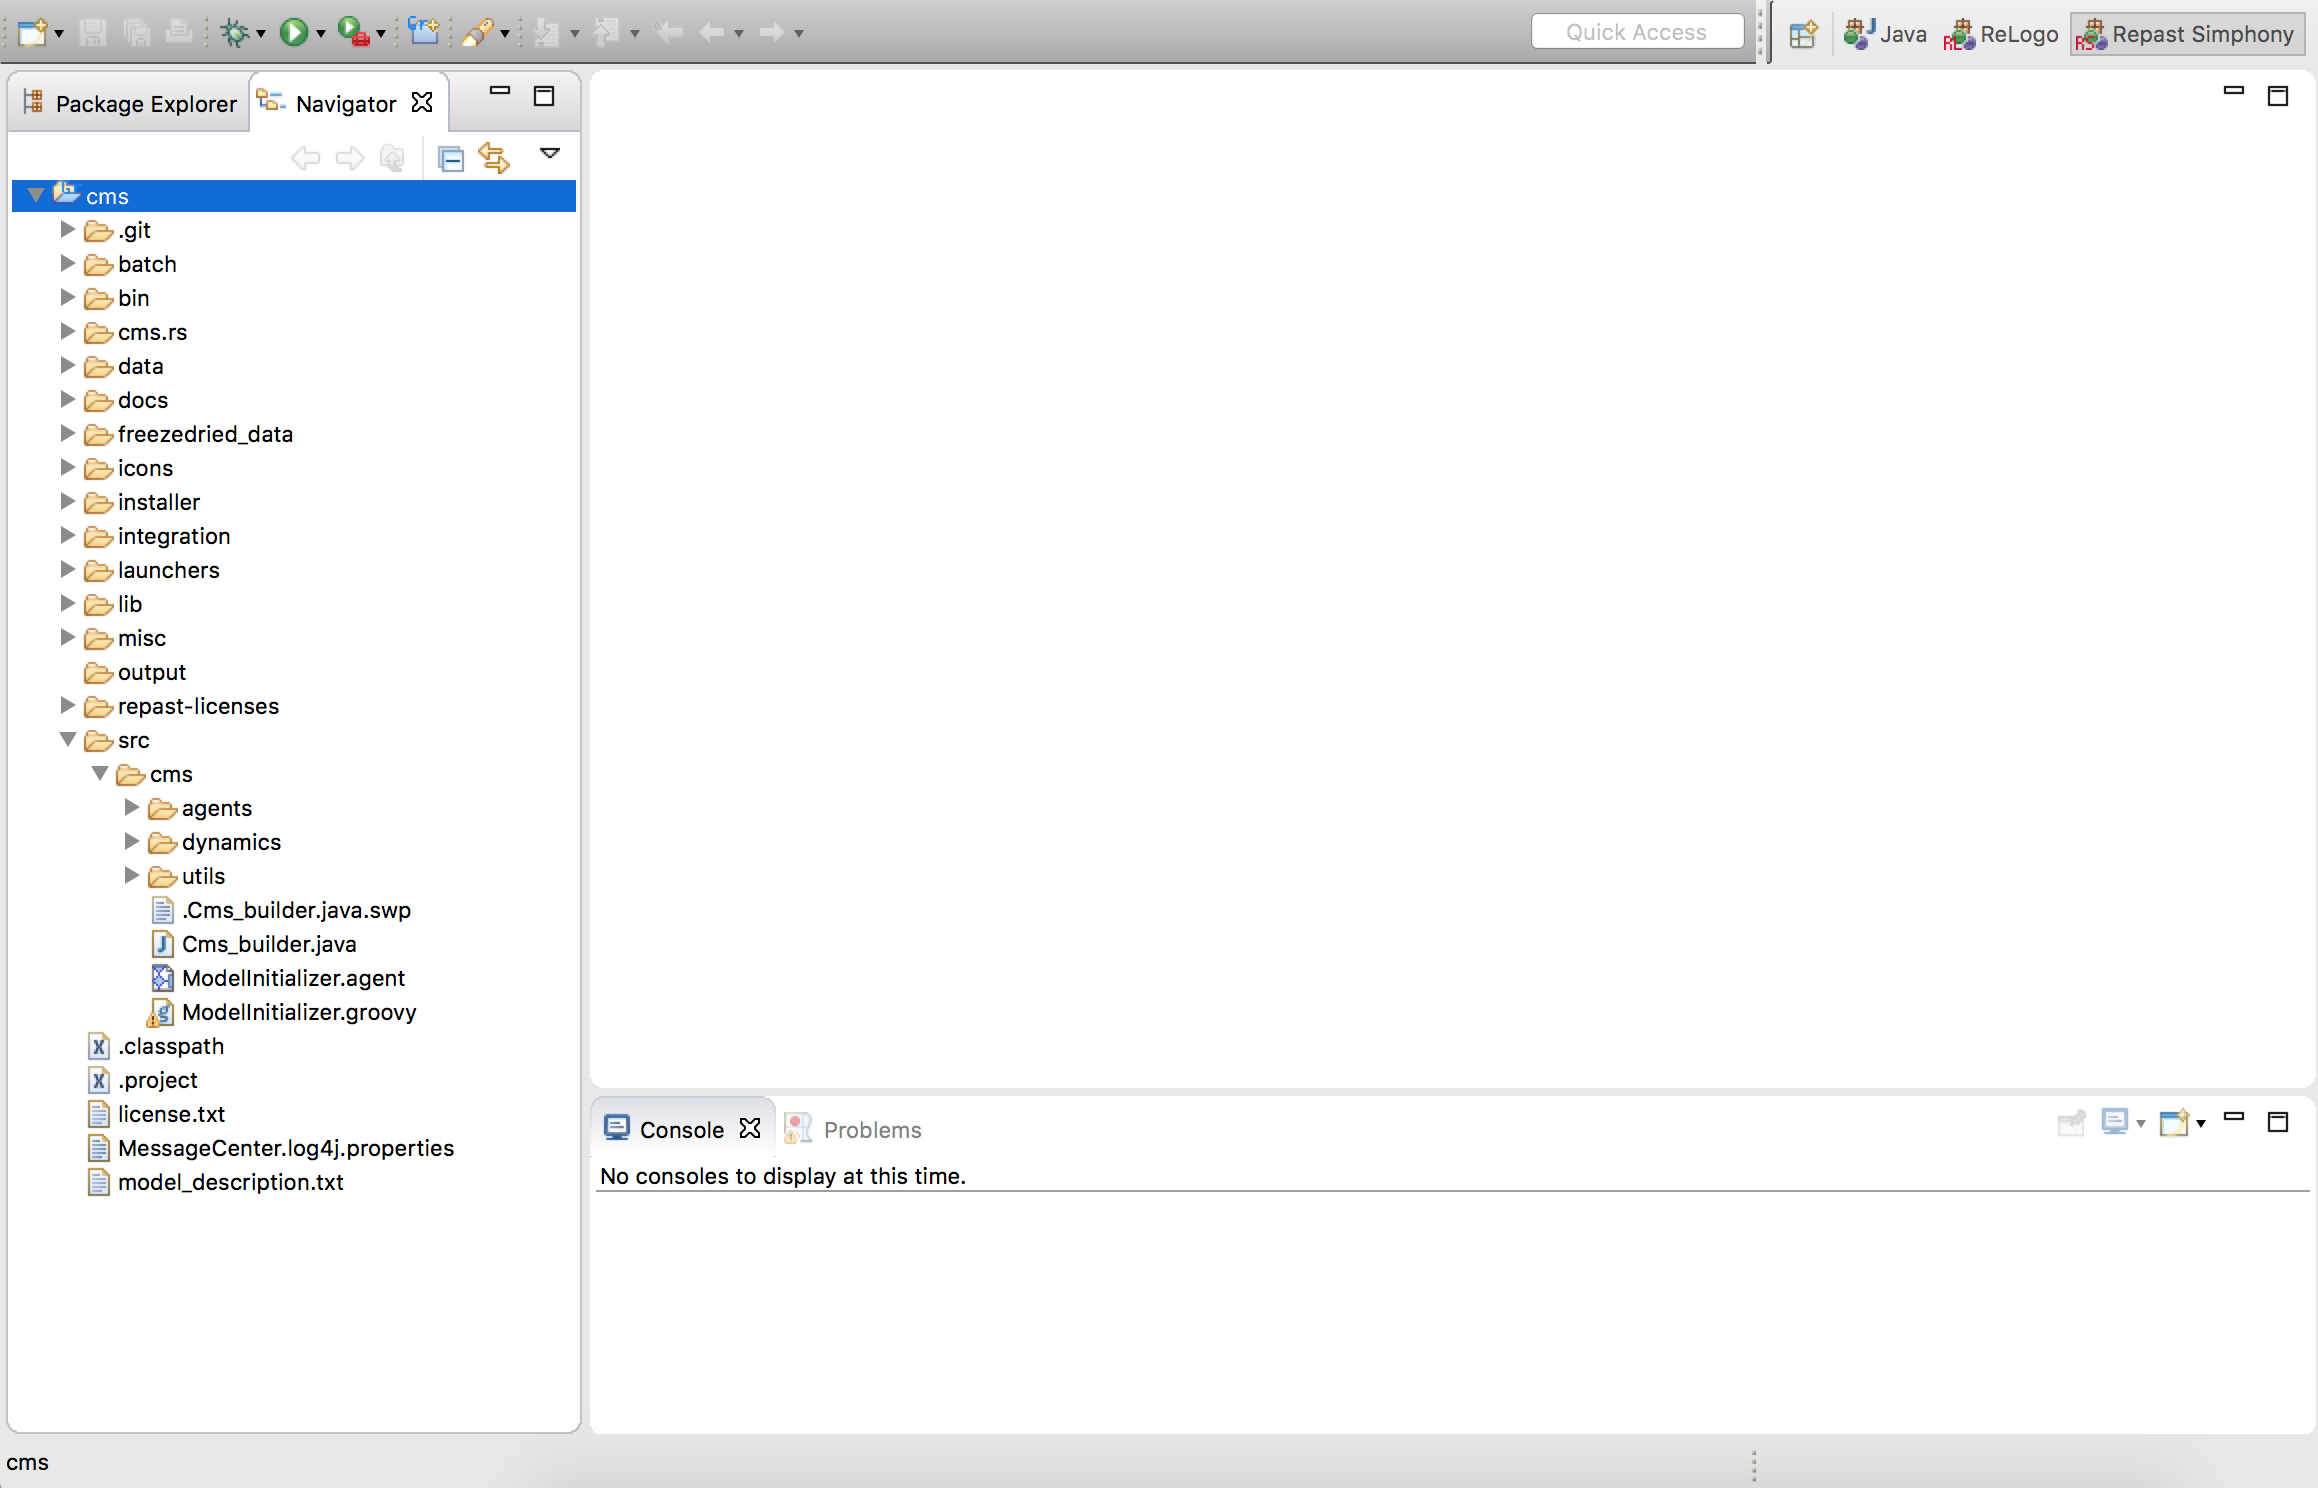
\includegraphics[scale=0.35]{fig_cms_rs_navigation1}

\vskip2mm

\subsubsection{Using a zip archive}

Point your browser to\\ 
\verb+https://github.com/ggiulion/cms+\\
Click on the ``clone or download'' button and choose ``download zip''.

This will download the \verb+cms-master.zip+ file in your system.

Unpacking it creates the cms-master folder.
Move the whole content of this folder in the cms RS project folder:\\  
\verb+/Users/coolcoder/Documents/workspace/cms/+\\
Choose to overwrite existing files and folders if you will be asked (this will merge folders). 

Now refresh eclipse (file $\rightarrow$ refresh).



\section{Testing the Installation}


There are two ways of running RS models: The GUI and the BATCH mode.

The GUI mode can be of great visual impact because several monitoring devices continuously updating during runtime can be added to the RS GUI window. The flip side of the coin is that these devices slow down simulation execution. Second, the simulation runs exclusively in a machine running an X server. Notwithstanding the GUI mode can be a valid tool during the model development, however when massive simulations are performed, the BATCH mode should be used instead. BATCH mode runs are faster because all the graphics elements are turned off. Furthermore, the absence of graphics makes it possible to run the model in parallel on several machines. It is worth saying that RS has very useful facilities for running a model in parallel.


Let us start this section from the very beginning i.e. with the eclipse software just opened and show how to run the model in GUI mode. 
We discuss the BATCH mode after the discussion on how to customize the model.

First of all, click on the down black arrow highlighted by the red circle in the following picture

\vskip2mm
\noindent

\includegraphics[scale=0.35]{fig_cms_rs_execution1}

After clicking, a menu opens as shown by the following figure. 

\vskip2mm
\noindent
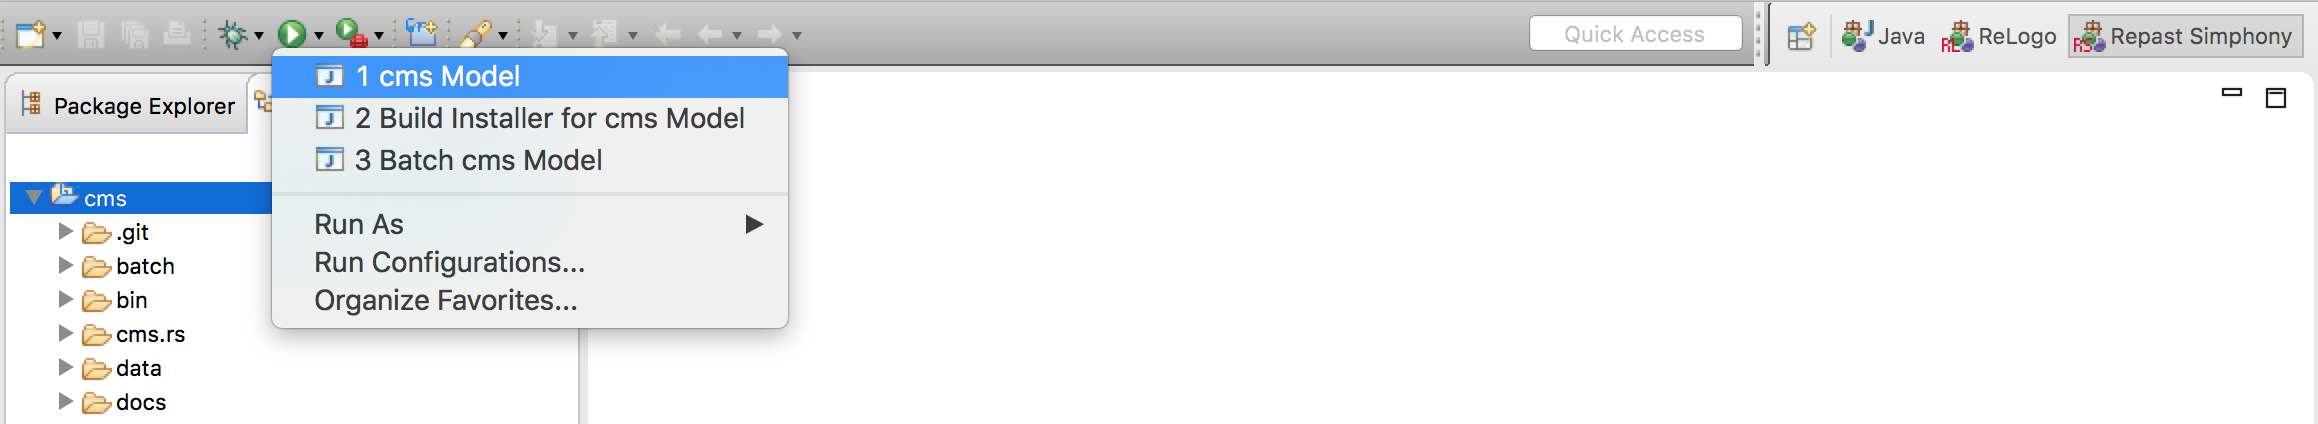
\includegraphics[scale=0.35]{fig_cms_rs_execution2}

\vskip2mm
The GUI execution is activated by clicking the \verb+cms Model+ item and after few seconds the model window will show up. Click the 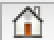
\includegraphics[scale=0.4]{fig_home} button, and you should see a well framed world map.
%, while the BATCH execution can be started by clicking the \verb+Batch cms model+.
%Check if Context is listed under the Data Loaders item of the scenario tree.

Use the RS GUI window intuitive buttons to interact with the simulation. A more detailed description on how to control the simulation is given at page 24 of the ``Repast Java Getting Started'' document available in RS web site.

Now the model has no dynamic monitoring graphical elements, so one can check the progress of the simulation watching at the tick count number in upper right corner of the RS GUI window or looking at the text output in the console panel of Eclipse window as shown in the following figure. 

\vskip2mm
\noindent
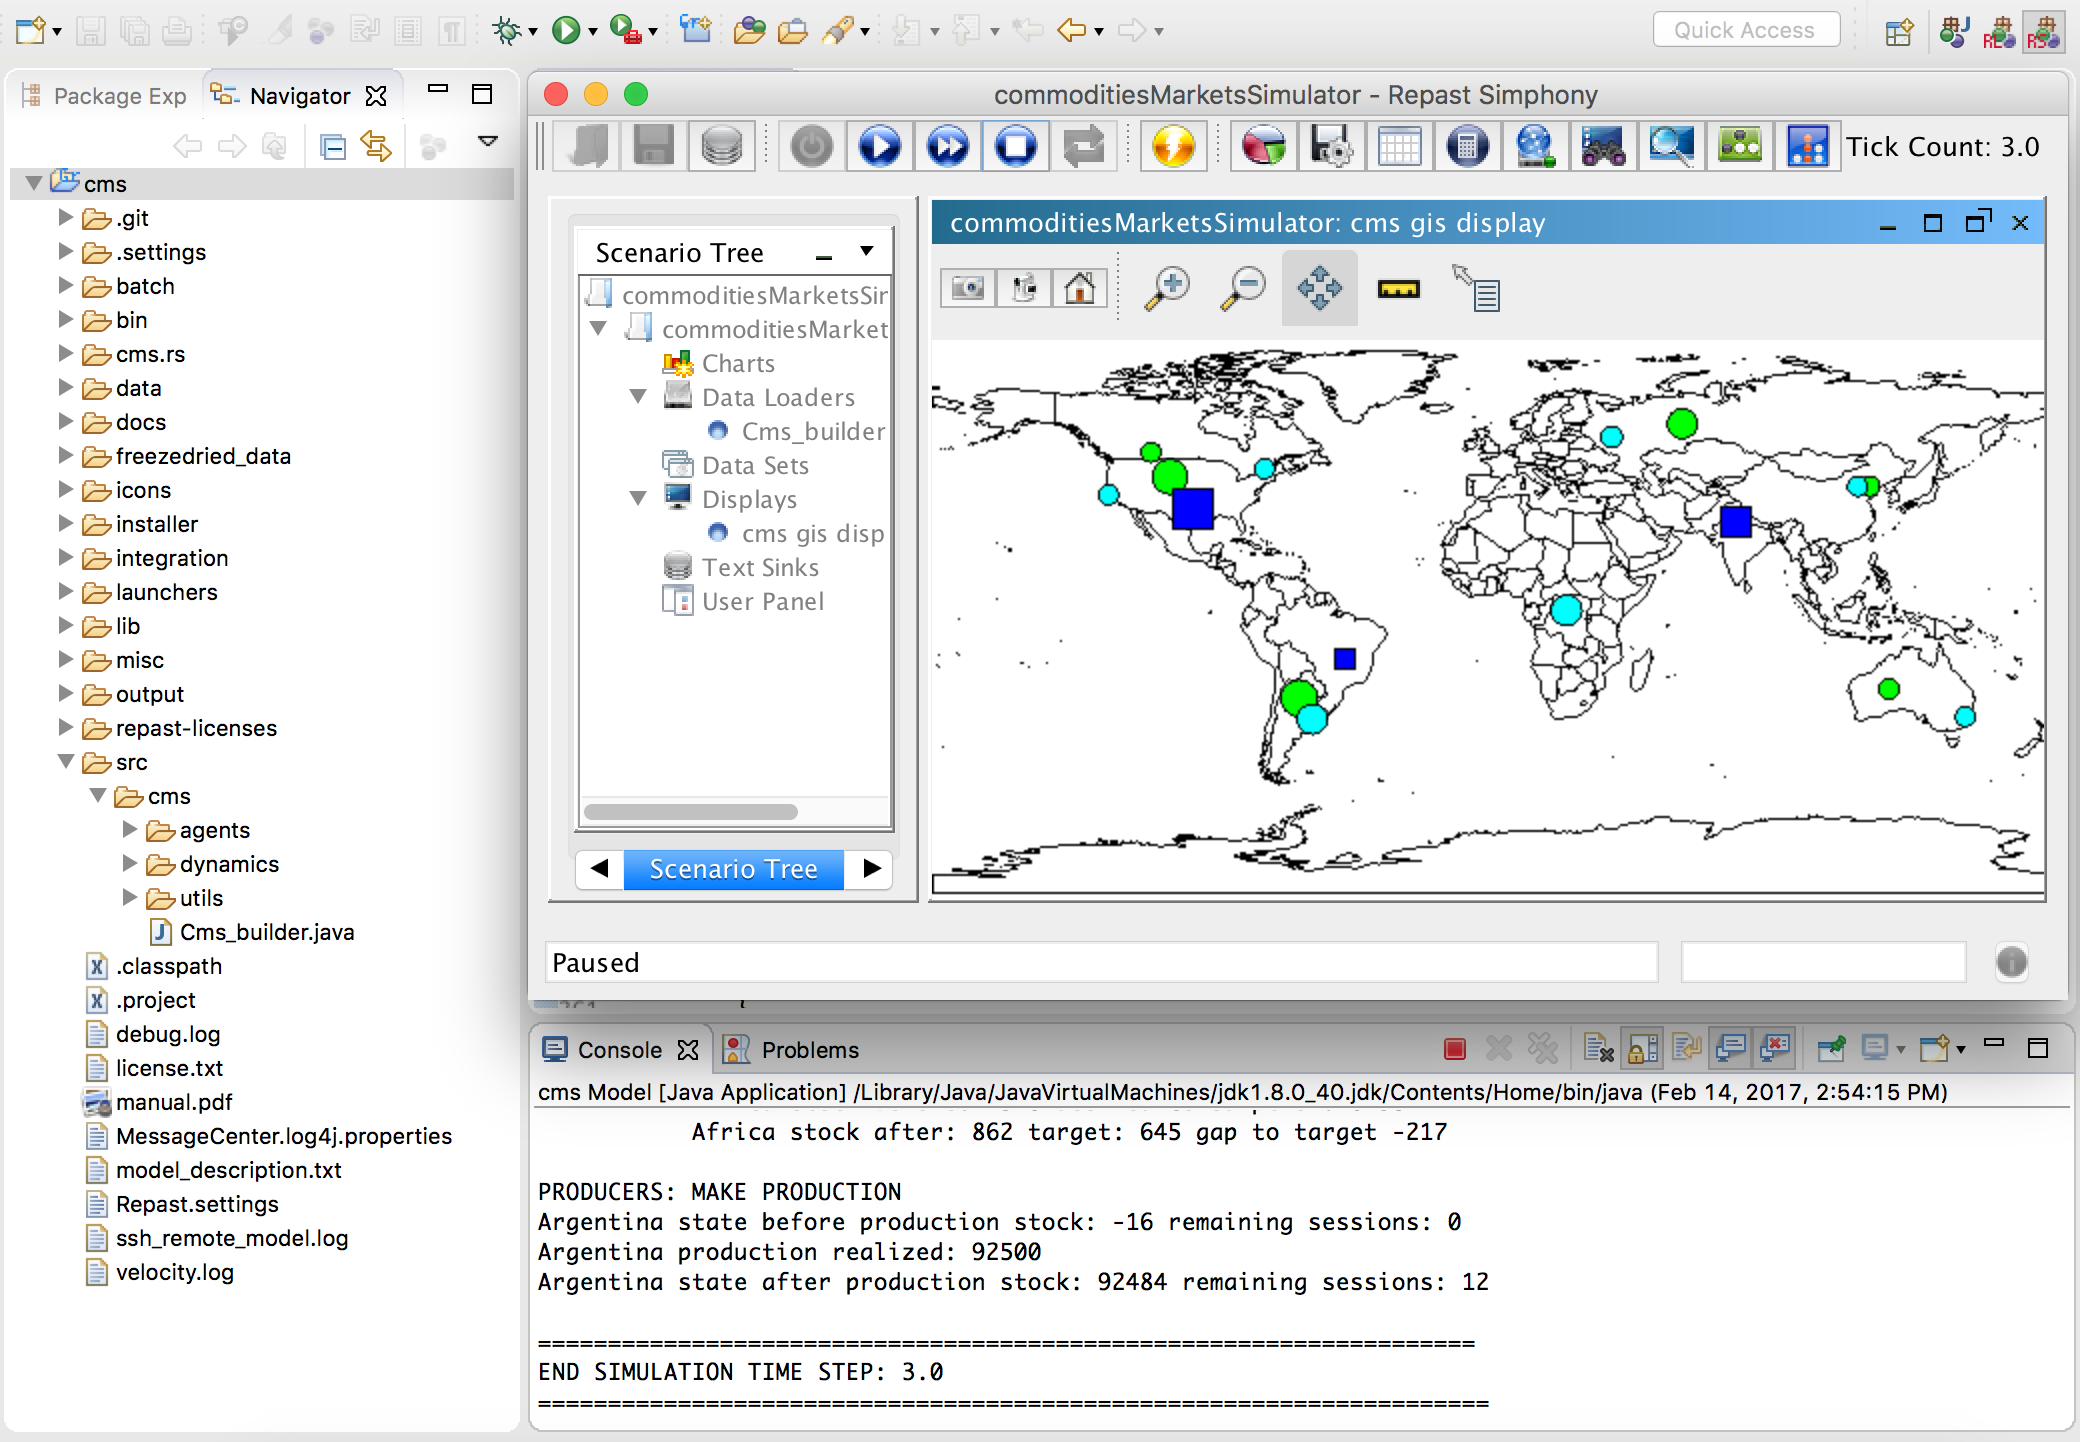
\includegraphics[scale=0.35]{fig_cms_rs_gui7}

\vskip2mm





\section{Customizing the simulation}\label{sec:initialization}
\subsection{Creation and configuration of agents}

As explained above, the model is populated by three types of agents: producers, buyers and markets.

The agents creation and configuration process is guided by three configuration files located in the scenario folder \verb+cms.rs+.
They are named after three agent types and have a comma separated values format. They are: \verb+producers.csv+, \verb+buyers.csv+ and \verb+markets.csv+.

Each line of these files (except the first one which is for headings) contains the information to setup an agent. The researcher can thus configure the simulation by writing these files.

We report hereafter examples of these files to show the fields needed in each of them.

\subsubsection{Producers}
An example of the \verb+producers.csv+ file is the following 

\begin{verbatim}
name,latitude,longitude,production share,markets,products,first production time
China,39.9390731,120.1172706,0.05,New Delhi,Product A,2
United States of America,43.01,-104.08,0.2,Dallas|Brasilia,Product A,1
Argentina,-27.9878842,-62.6300825,0.3,Brasilia,Product A,3
Russian Federation,60.02,60.04,0.15,New Delhi,Product A,4
Canada,50.8725518,-110.1561254,0.05,Dallas,Product A,6
Australia,-24.9872587,126.1857131,0.05,New Delhi,Product A,8

\end{verbatim}

After loading this file, the simulator creates six producers. Note that the last line of the file must be empty.
As one can understand from headings (first line), each line contains the following information:
\begin{itemize}
	\item the producer's name,
	\item the producer's latitude,
	\item the producer's longitude,
	\item the producer's production share \gls{par:s_p}. Together with the global production \gls{par:P0}, is used to compute the producer's average production \gls{var:Y_{b,0}},
	\item the markets where the producer sells. The \verb+|+ character is used when more than one market is specified (see for example the United States configuration line). The program creates a session for the producer in each specified market,
	\item the products obtained by the producer. Even in this case, the \verb+|+ can be used to signal that the producer obtains different products. However, in case the researcher is interested in setting up a model with more than one product, s/he has to modify the code to model gents' choice concerning the supply and demand of these different products,
	\item the first production time variable. It is introduced to account for production that are obtained in different seasons across producers. Together with the \gls{par:tau} parameter, this enable the simulator to handle non-continuous production processes such as those of agriculture products. As an example we can have a yearly production cycle for each producer, but some producer obtain the product in June while other in December.
\end{itemize}

\subsubsection{Buyers}
An example of the \verb+buyers.csv+ file is the following 

\begin{verbatim}
name,latitude,longitude,demand share,demand curve intercept,demand curve slope
China,39.9390731,116.1172706,0.1,5000,500
United States of America,37.1957928,-123.7650303,0.10,5000,500
Argentina,-34.6155729,-58.5033604,0.2,5000,500
Russian Federation,55.7498598,37.3523163,0.15,5000,500
Canada,45.5581968,-73.8516467,0.1,5000,500
Australia,-33.8474027,150.6517756,0.1,5000,500
Africa,0.1659234,22.938695,0.10,5000,500

\end{verbatim}

After loading this file, the simulator creates seven buyers. Note that the last line of the file must be empty.
As one can understand from headings (first line), each line contains the following information:
\begin{itemize}
	\item the buyer's name. This is matched against the first column of the \verb+producers.csv+ file to find out if the buyer is associated to a producer or not. 
		According to our assumption, all the producers have an associated buyer, but the reverse is not true. Therefore, the number of lines in the \verb+buyers.csv+ file equals or is higher than those of the \verb+producers.csv+ file.  In the case of the configuration file reported above, the first six lines specify buyers associated to producers. The seventh line (\verb+Africa+) has not an associated producer. This buyer will never forbid import of the commodity during simulation runs.
	\item the buyer's latitude,
	\item the buyer's longitude,
	\item the buyer's demand share \gls{par:s}. This is used to setup the desired consumption (\gls{var:C^d_b}) and the desired level of inventories (\gls{var:I^d_b}) as explained above. The level of inventories at the beginning ($I_{b,0}$) is set at the desired level, then they evolve as explained above.
	\item the intercept of the demand curves (\gls{par:barDb0}). This is used to setup the initial level of the intercept in each market session. As explained above, the intercepts evolve during the simulation.
	\item the slope of the demand curves (\gls{par:d_{b}}). This remains the same in all the market sessions during simulation runs.
\end{itemize}

\subsubsection{Markets}
An example of the \verb+markets.csv+ file is the following 

\begin{verbatim}
City,latitude,longitude,exchanges share
Brasilia,-15.6308631,-47.9994128,0.1
Dallas,32.8209296,-97.0115313,0.2
New Delhi,28.5275198,77.0688989,0.15

\end{verbatim}

After loading this file, the simulator creates three markets. Note that the last line of the file must be empty.
As one can understand from headings (first line), each line contains the following information:
\begin{itemize}
	\item the market's name. This is matched against the fifth column of the \verb+producers.csv+ file when market sessions are created.
	\item the market's latitude,
	\item the market's longitude. This is used to determine the order of market opening in case the model has two or more markets.
	\item the market's exchange share. This is used for graphical uses.
\end{itemize}


\subsection{Output}
This subsection shows how to add graphical elements to the model interface or to make the model able to save data.

\subsubsection{Adding a GIS display}
The models comes with a gis display showing a world map. We will first delete it and make it again in order to show how the user can configure her/his own display.

Right click the \verb+cms gis display+ in the scenario tree and choose delete to remove the display. Now we will build again the display. 

Right click the Display item in the Scenario tree and click on Add display as shown in the following figure

\vskip2mm
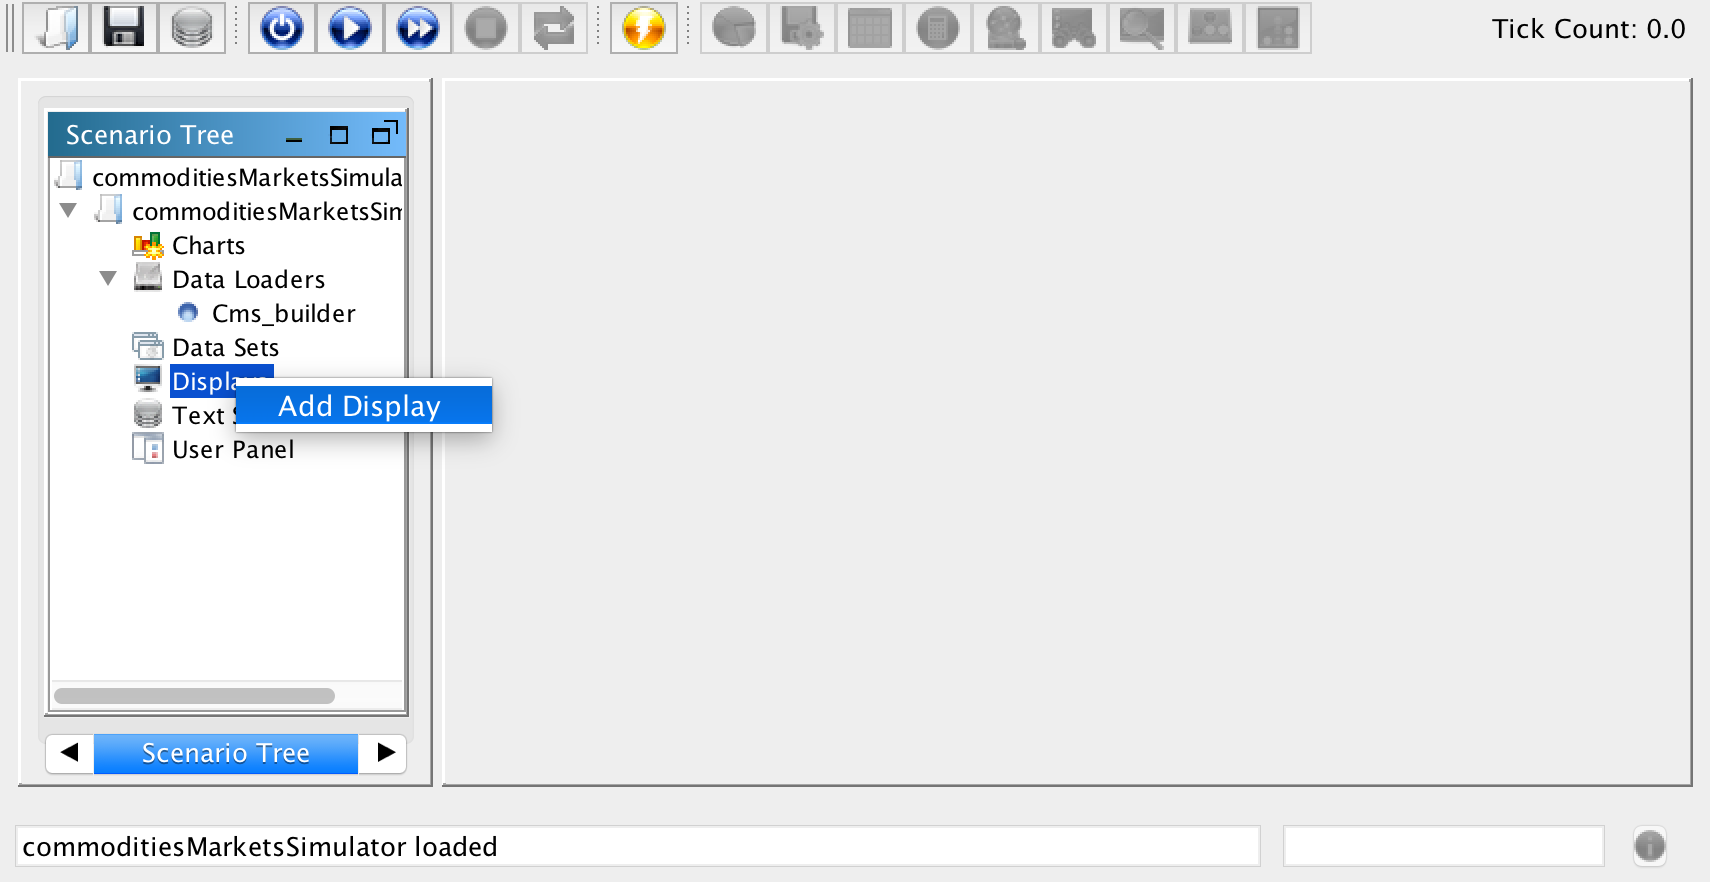
\includegraphics[scale=0.35]{fig_cms_rs_gis1}

\vskip2mm
a wizard opens. Edit the display name, chose the GIS option and move the Geography item from the left to the right

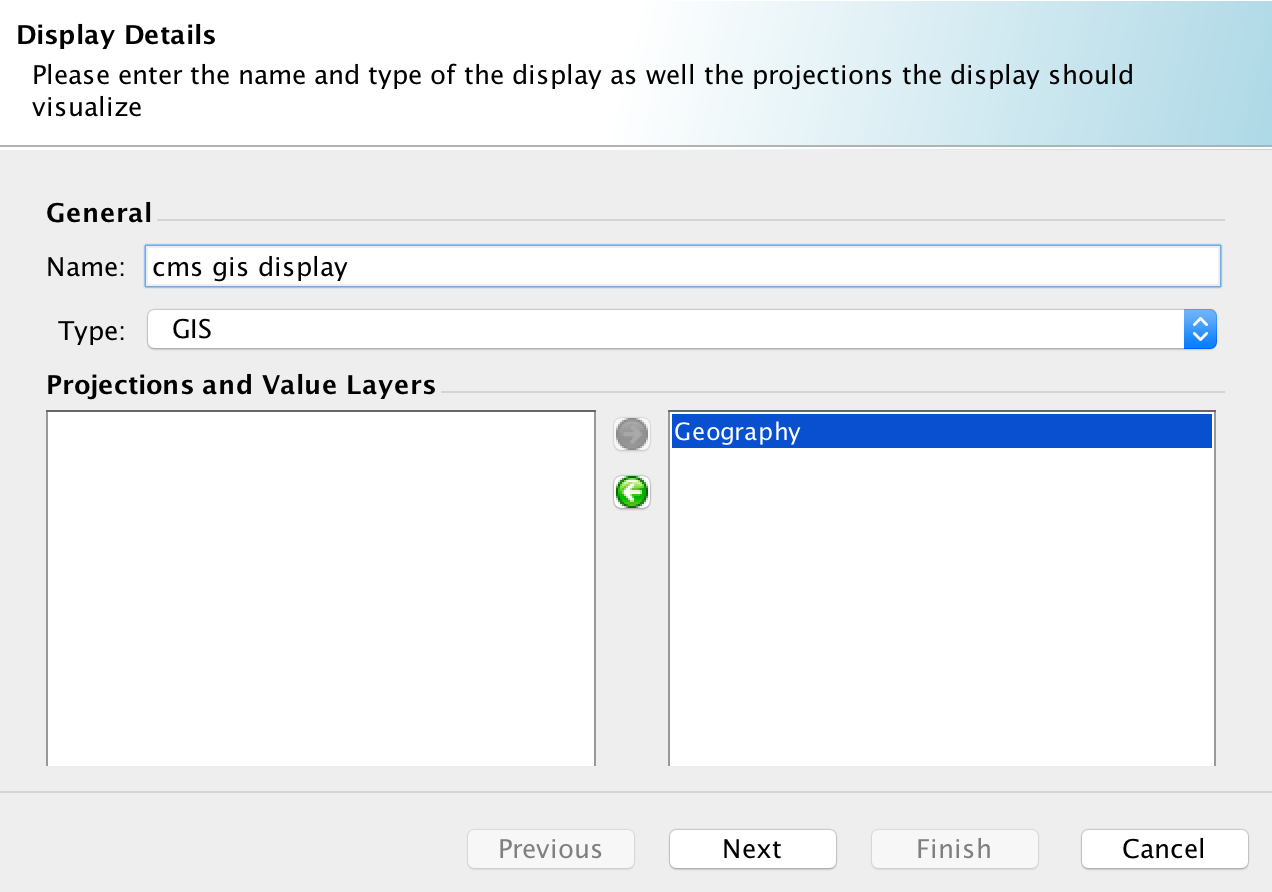
\includegraphics[scale=0.35]{fig_cms_rs_gis2}

Click the next button and move the agents to be displayed from the left to the right

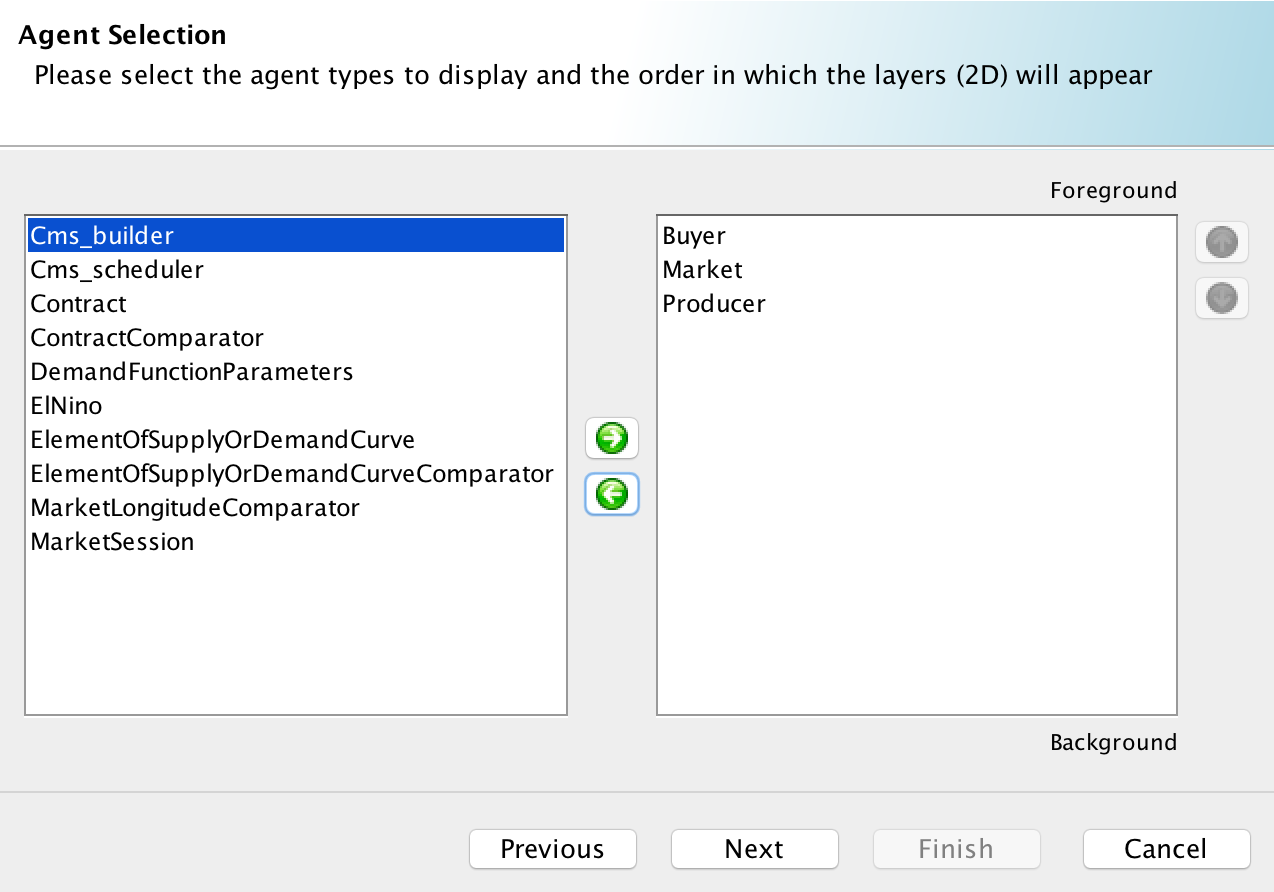
\includegraphics[scale=0.35]{fig_cms_rs_gis3}

By clicking the next button a new window opens. It gives the possibility to customize the appearance of each type of agents on the display and to add additional elements.

To edit the appearance of an agent, select an agent type and click on the edit icon which is highlighted in the next figure (in the case of the figure the appearance of Buyers will be configured)

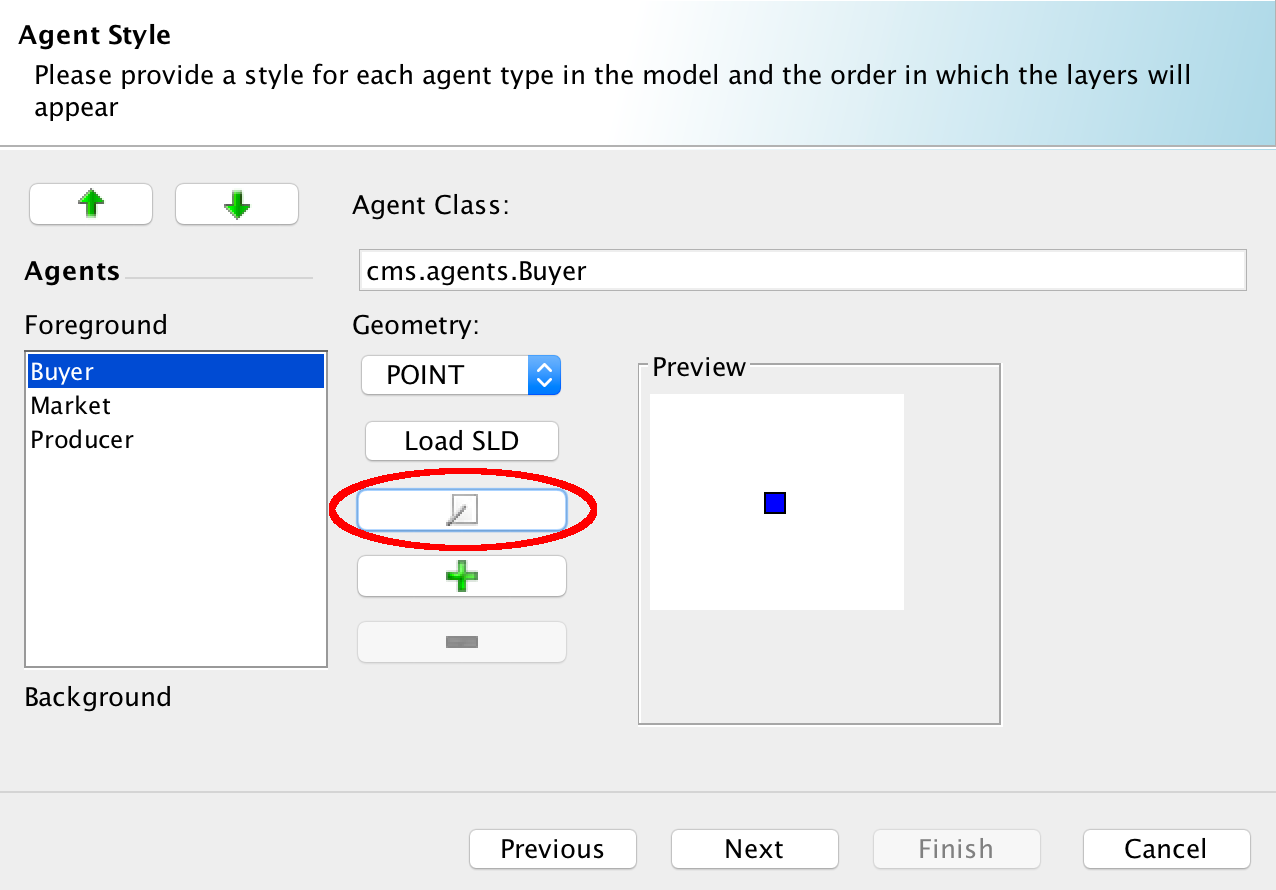
\includegraphics[scale=0.35]{fig_cms_rs_gis4a}

Click on the button highlighted in the next figure to add elements

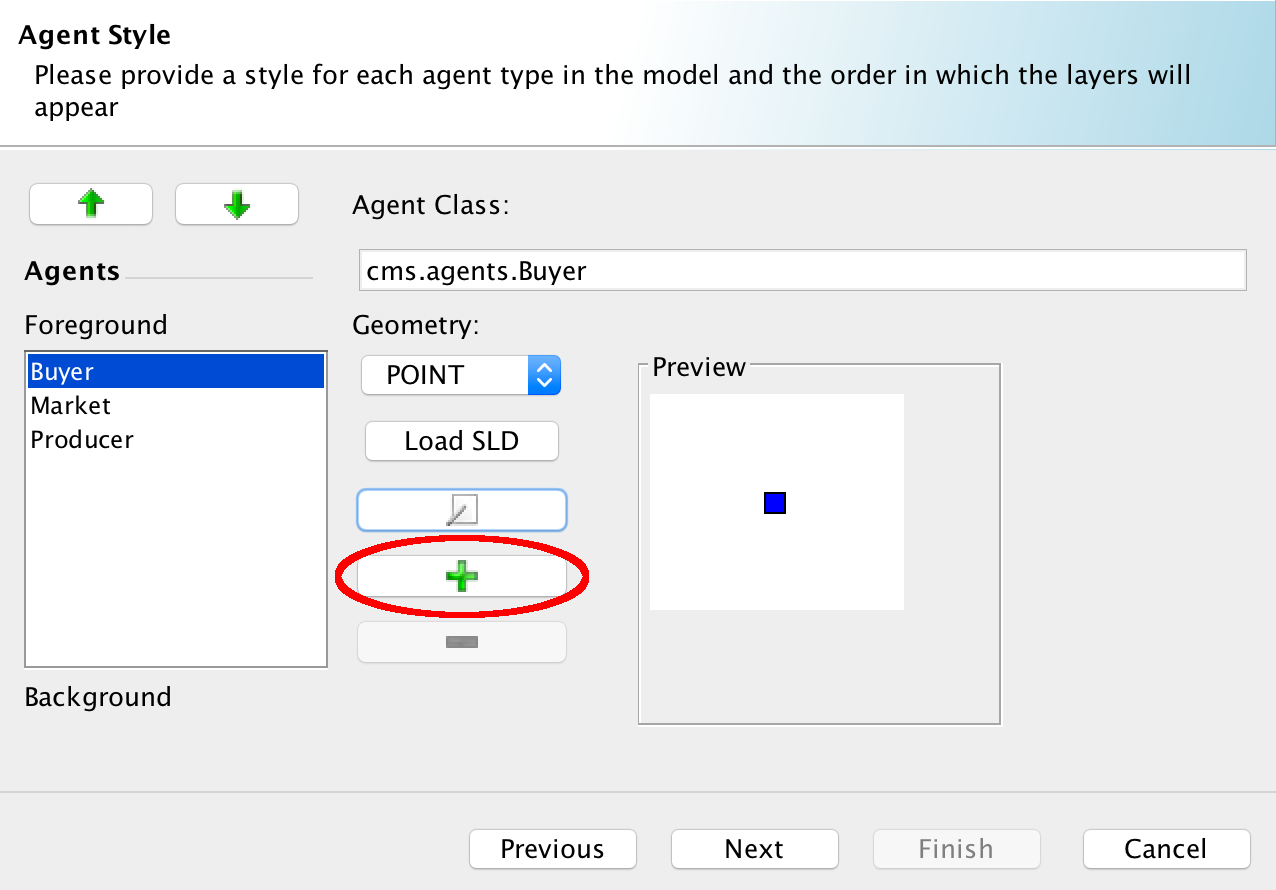
\includegraphics[scale=0.35]{fig_cms_rs_gis4b}

We will show hereafter how to add a background showing a geographic zone. First of all, a shapefile of the zone is needed.  
Shapefiles are often available for downloaded in Internet. Some shapefiles downloaded from \url{http://www.naturalearthdata.com/}\footnote{
	in particular they relate to world maps available at \url{http://www.naturalearthdata.com/downloads/50m-cultural-vectors/} or \url{http://www.naturalearthdata.com/downloads/10m-physical-vectors/}.} are already included in the \verb+data+ folder.

By clicking on the button highlighted in the figure above, a file browser opens. Manage to select your shapefile. In the following figure, a shapefile in the \verb+data+ folder is selected

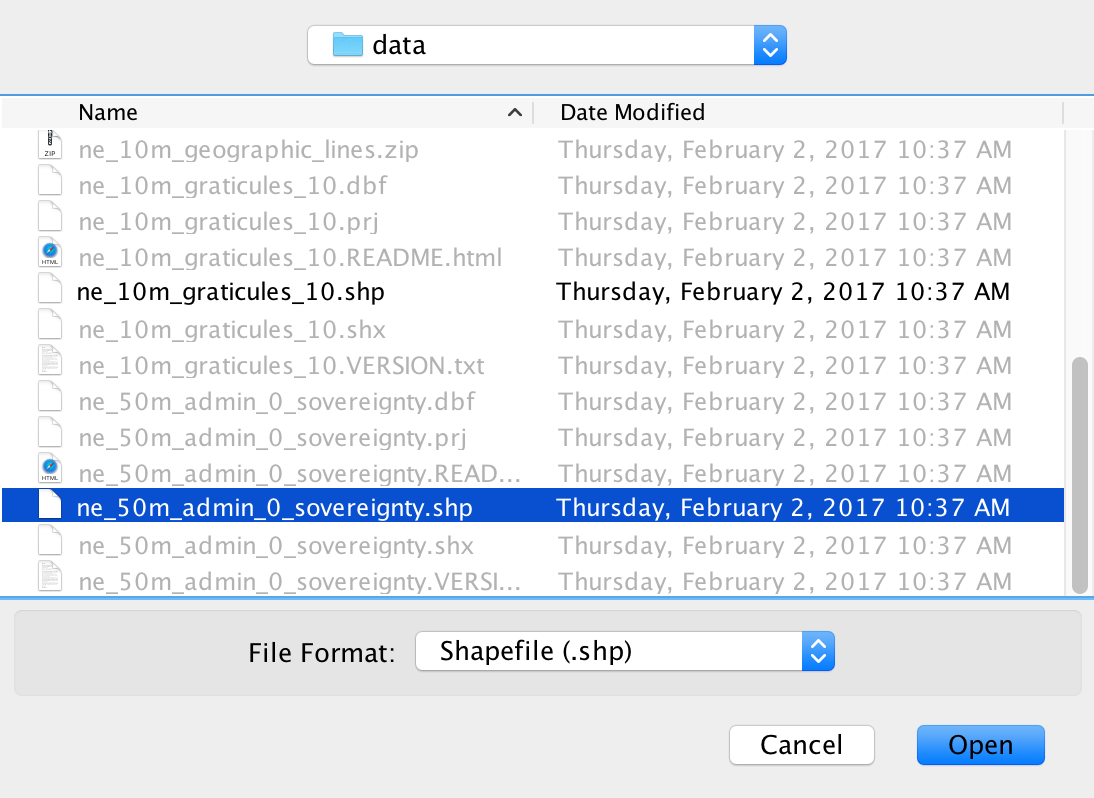
\includegraphics[scale=0.35]{fig_cms_rs_gis6}

Clicking the open button, an additional element appears in the agent style window as shown in the following figure.

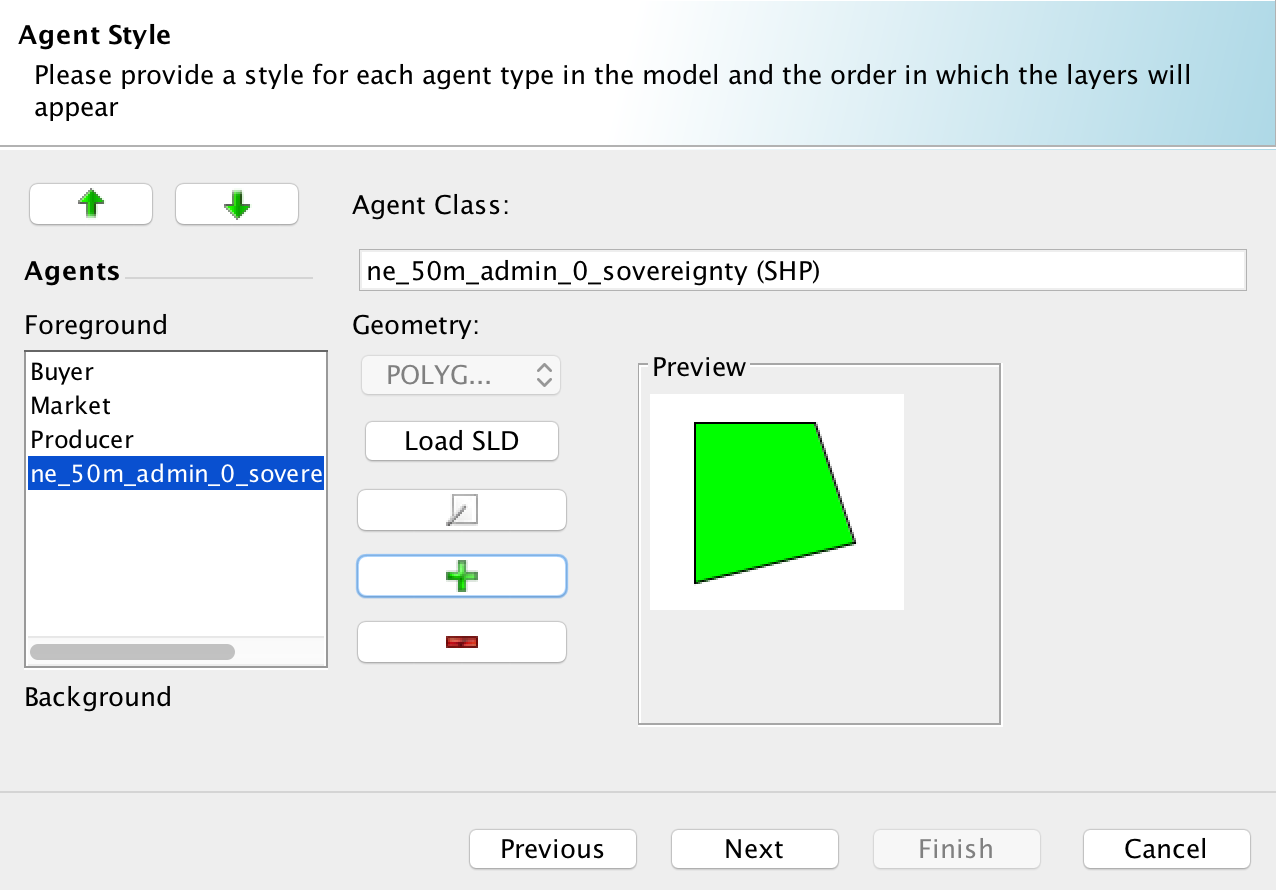
\includegraphics[scale=0.35]{fig_cms_rs_gis7}

Edit this additional element if you want to customize it, and then click the next button. The following window opens. Refer to the RS documentation to customize these parameters or accept the proposed ones.

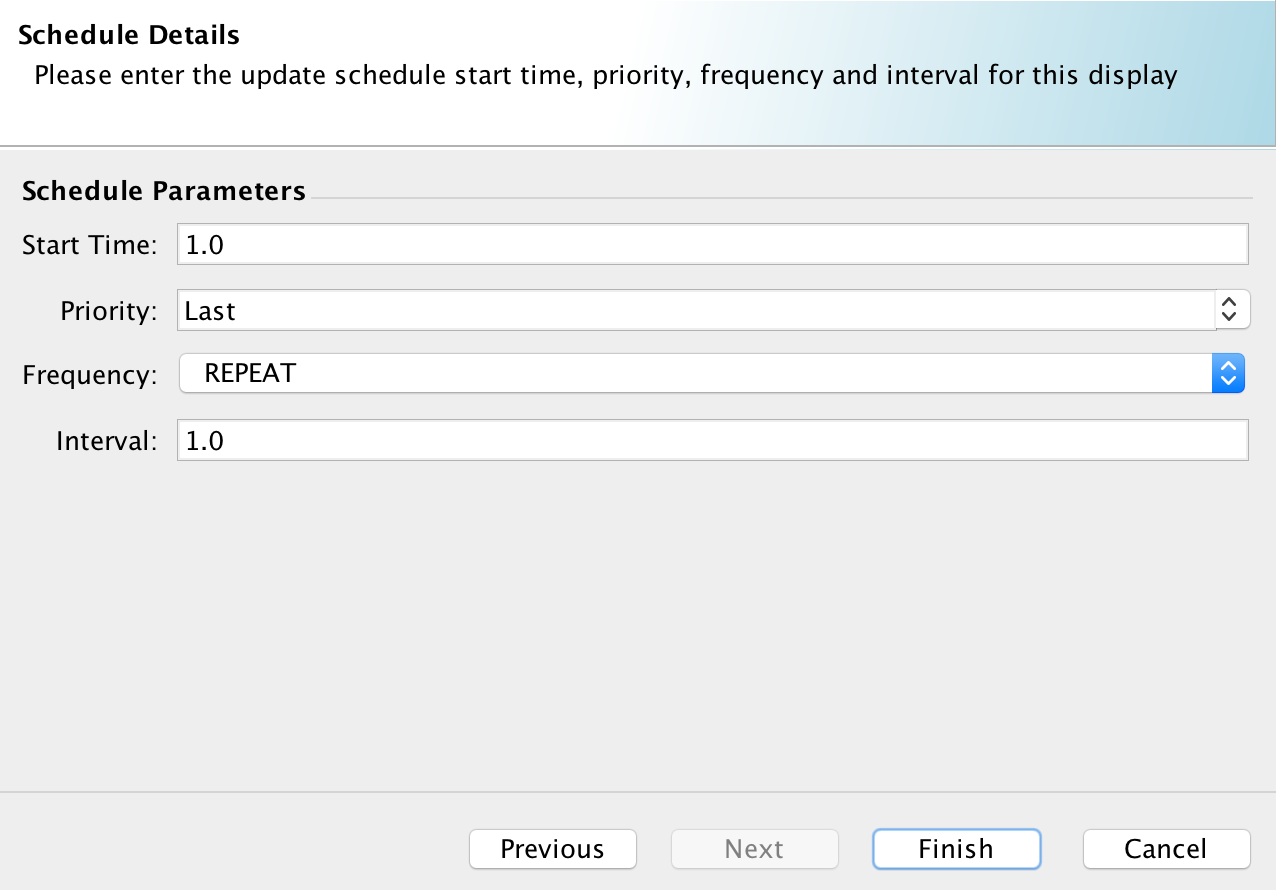
\includegraphics[scale=0.35]{fig_cms_rs_gis8}

By clicking the finish button the display item appears in the scenario tree as shown in the figure below

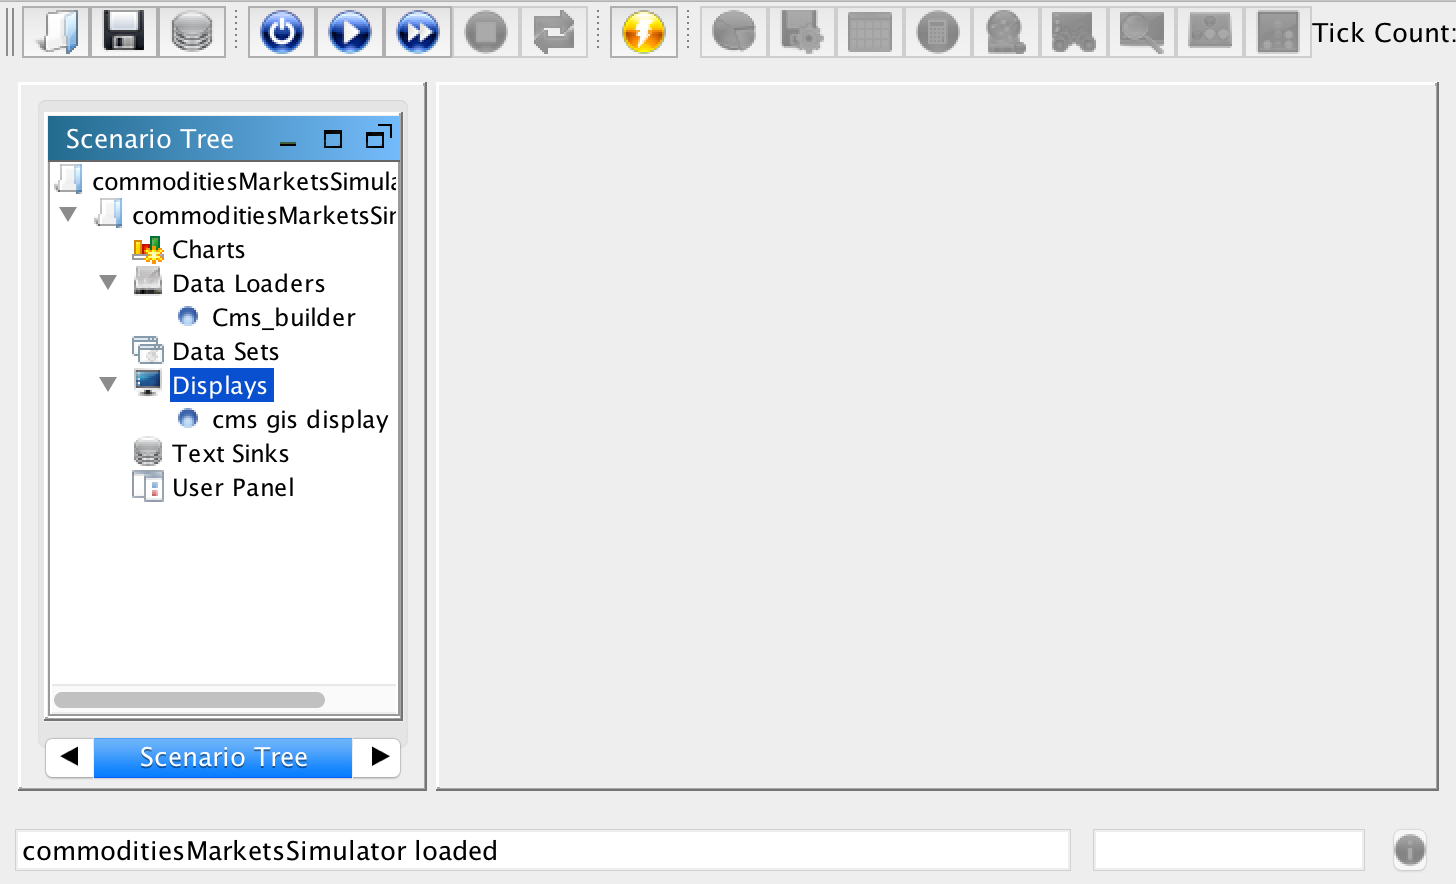
\includegraphics[scale=0.35]{fig_cms_rs_gis9}

Save the changes to the scenario tree by clicking the floppy disk image.

Now, clicking the Step Run button (highlighted in red in the following figure), the display will show up after few seconds. If the map is not centered in the windows, click 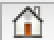
\includegraphics[scale=0.4]{fig_home} button to frame it. The following figure shows the final outcome  

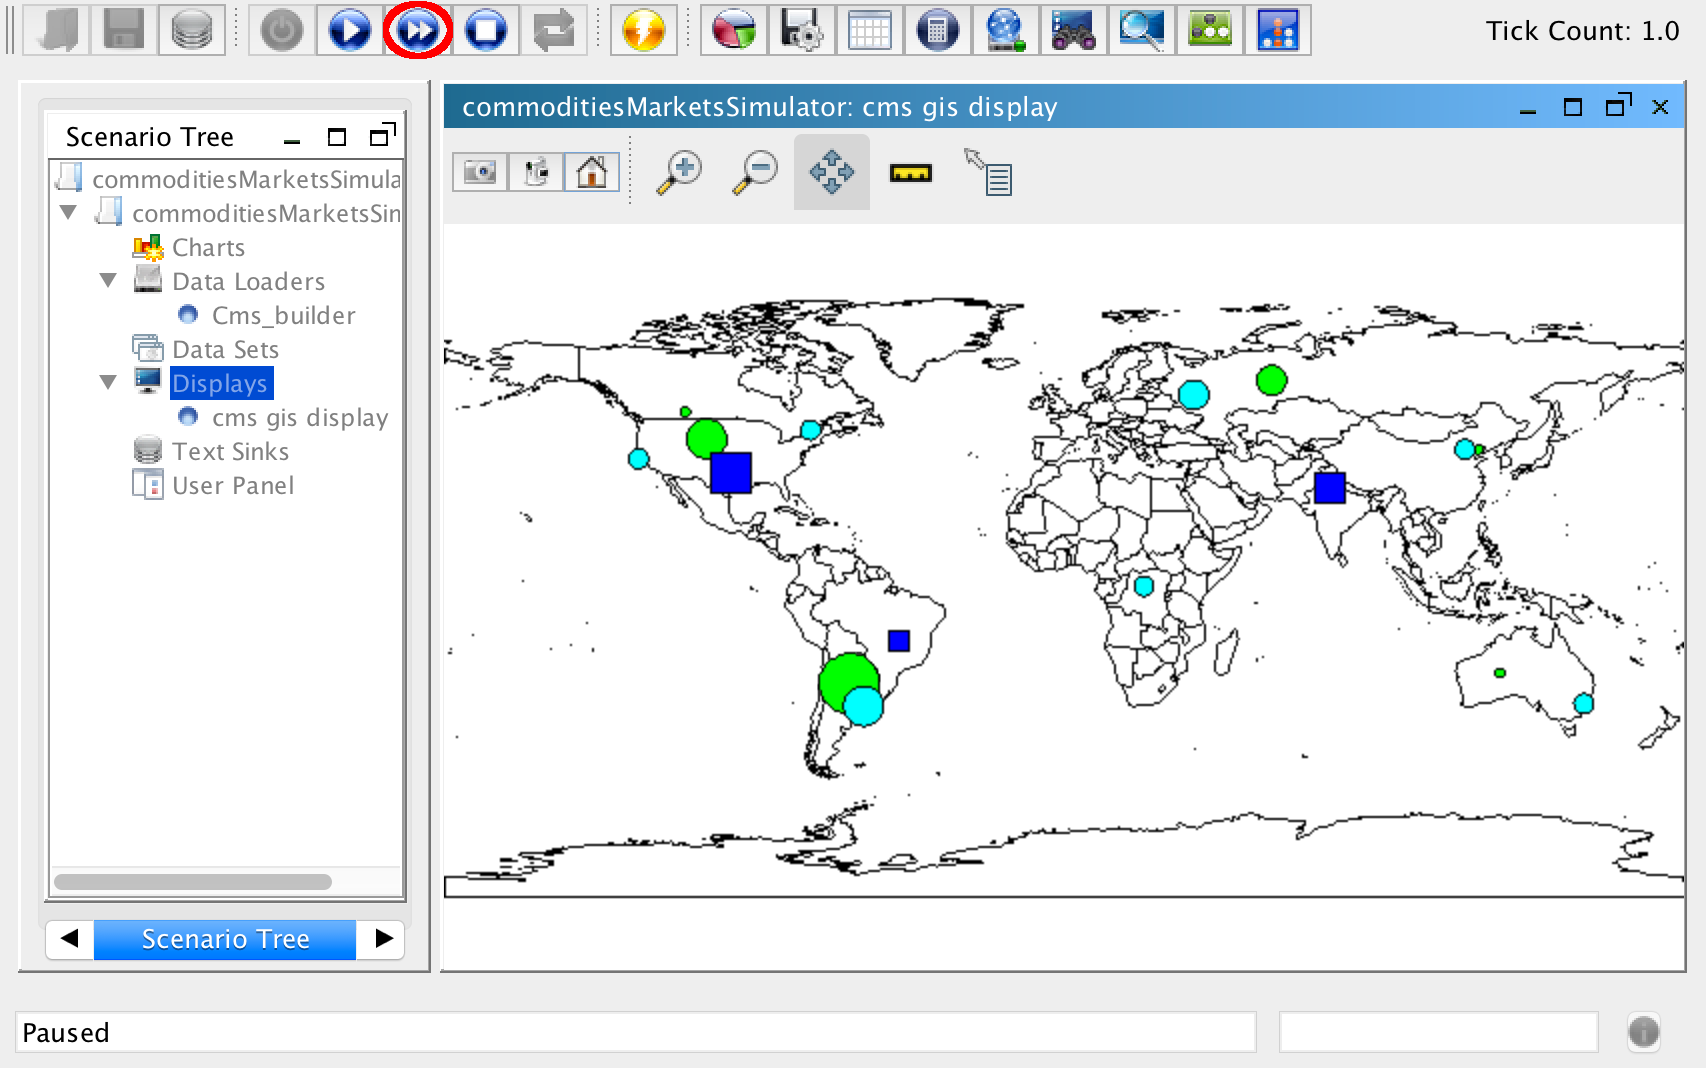
\includegraphics[scale=0.35]{fig_cms_rs_gis10}

In the figure above, the following customization are used:
\begin{itemize}
	\item producers are represented by green circles whose size is proportional to the production share specified in the \verb+producers.csv+ file;
	\item buyers are represented by light blue circles whose size is proportional to the demand share specified in the \verb+buyers.csv+ file;
	\item markets are represented by blue squares whose size is proportional to the exchanges share specified in the \verb+markets.csv+ file.
\end{itemize}


\subsubsection{Adding charts and data sinks}

These features can be added by managing the scenario tree displayed in the model GUI. The process is similar to the one described above for the display.

We will briefly describe this process pointing the reader to the RS documentation\footnote{In particular, the document describing data collection available at \url{https://repast.github.io/docs/DataCollection.pdf} is recommended.} for a more detailed description. 

Charts and Data Sinks take Data Sets as an input. Therefore, Data Sets have to be created first.

To create a data set, right click the corresponding item in the scenario tree and click on Add data set

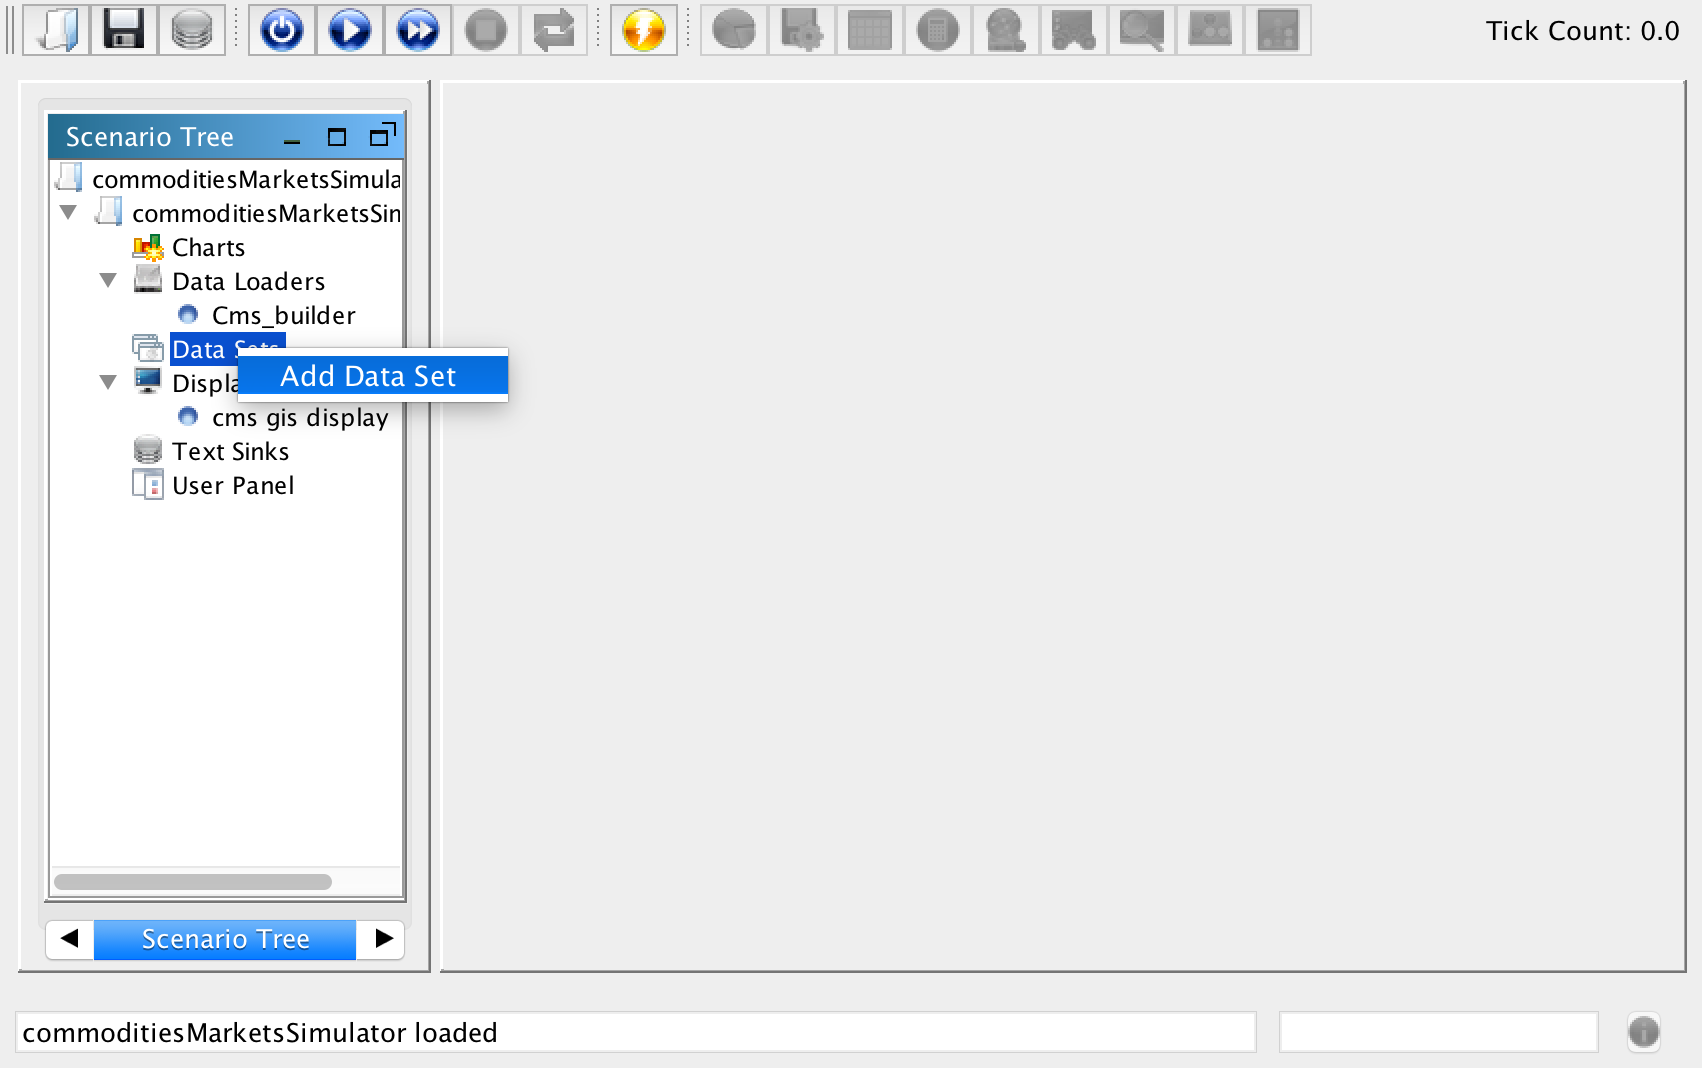
\includegraphics[scale=0.35]{fig_cms_rs_data1}

The wizard for creating the data set opens. Suppose now we want to gather data from all the market sessions. In the first wizard window displayed below we name the dataset \verb+market sessions dataset+ and inform the program that it is a Non-aggregate data set

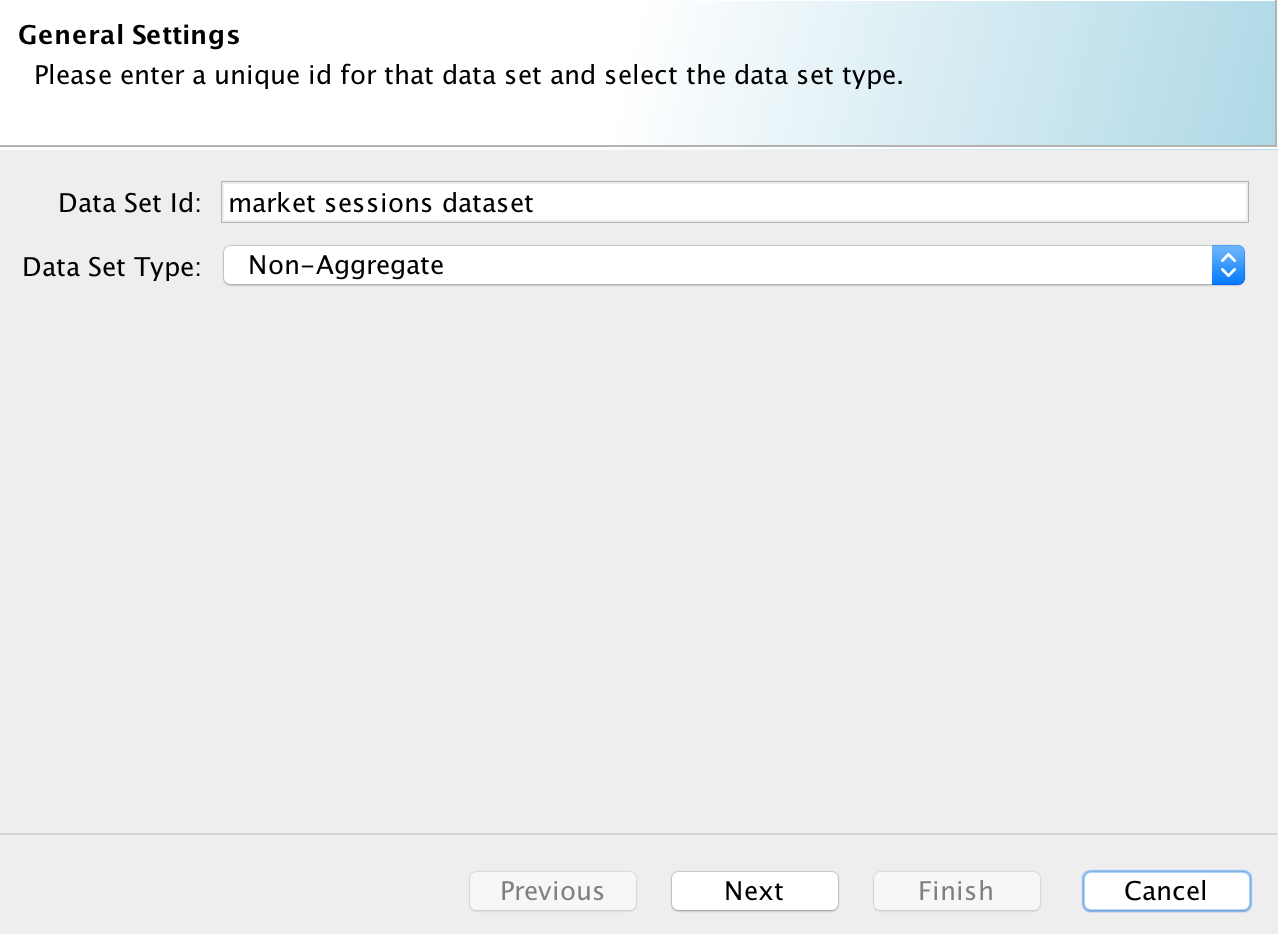
\includegraphics[scale=0.35]{fig_cms_rs_data2}

The following window allows to select the variables to be included in the data set. There are three tabs in this window. The first one (\verb+Standard Sources+) lists the variable made available by RS. The second one (\verb+Method Data Source+) allows to add new variable obtained using get methods of the chosen class. While the third one is for more advanced uses. The following figure shows the second tab, where the market description, the market price and the exchanged quantity are added to the data set 

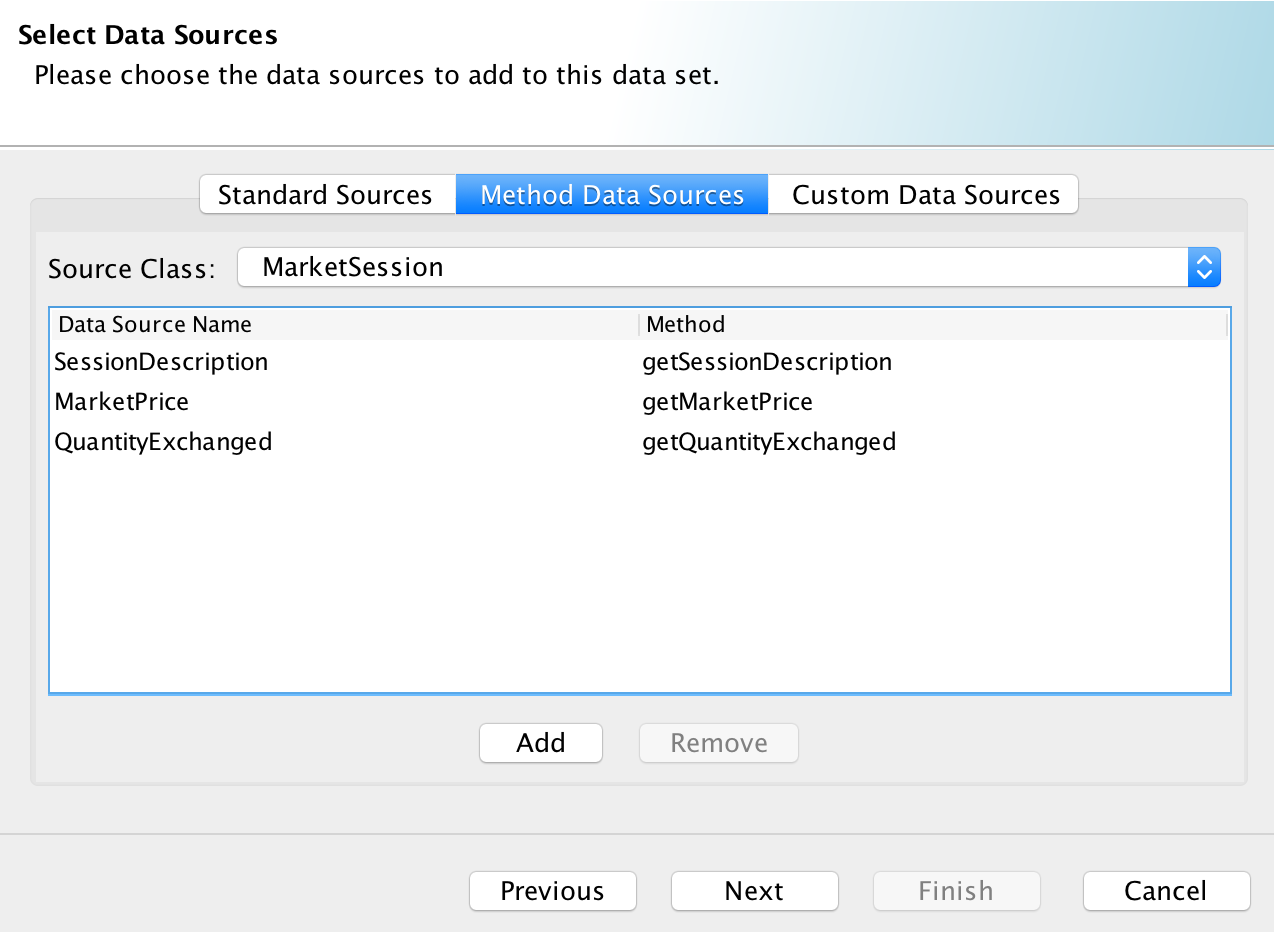
\includegraphics[scale=0.35]{fig_cms_rs_data3}

Once all the wizard steps are performed, the new dataset appears in the scenario tree as shown in the following figure

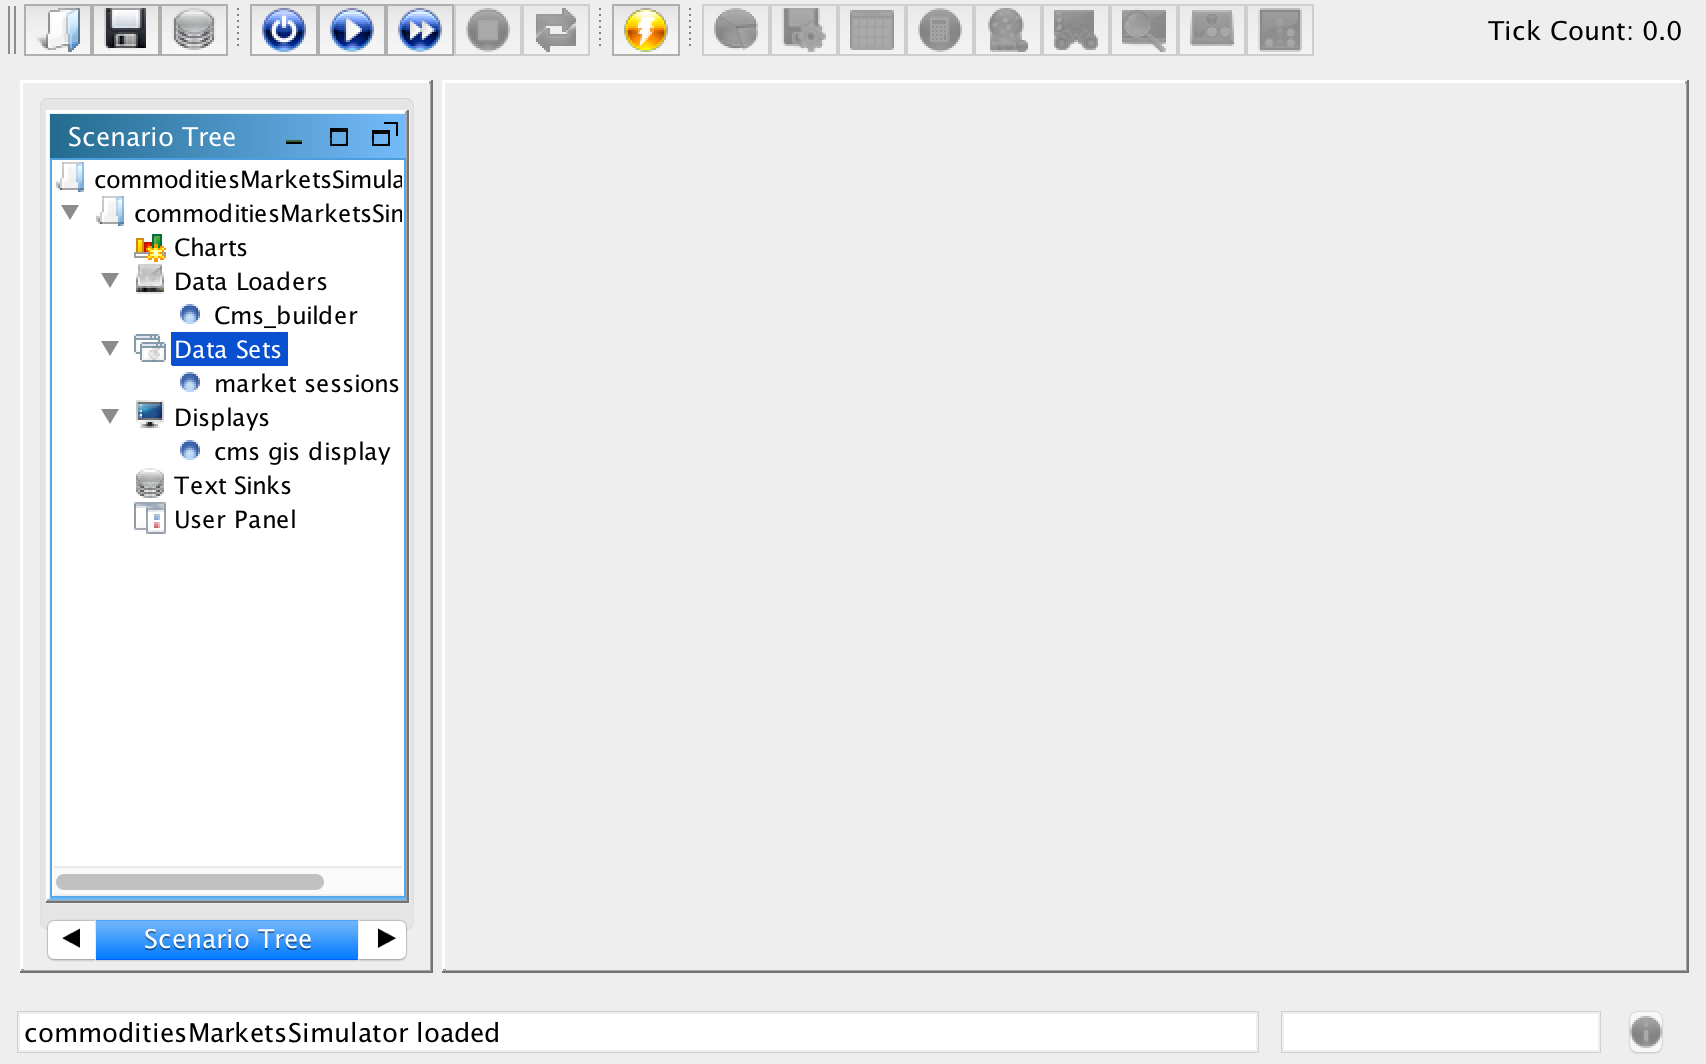
\includegraphics[scale=0.35]{fig_cms_rs_data4}

Now that we have a dataset, we can use its variables to chart data or to record them in a file (sink them). 

To create a new time series chart, start the corresponding wizard by right clicking the charts item in the scenario tree and select the time series option.
The chart name can be edited and the data set must be chosen among those created with the previously described procedure. The data set \verb+market sessions dataset+ previously created is selected in the following figure: 

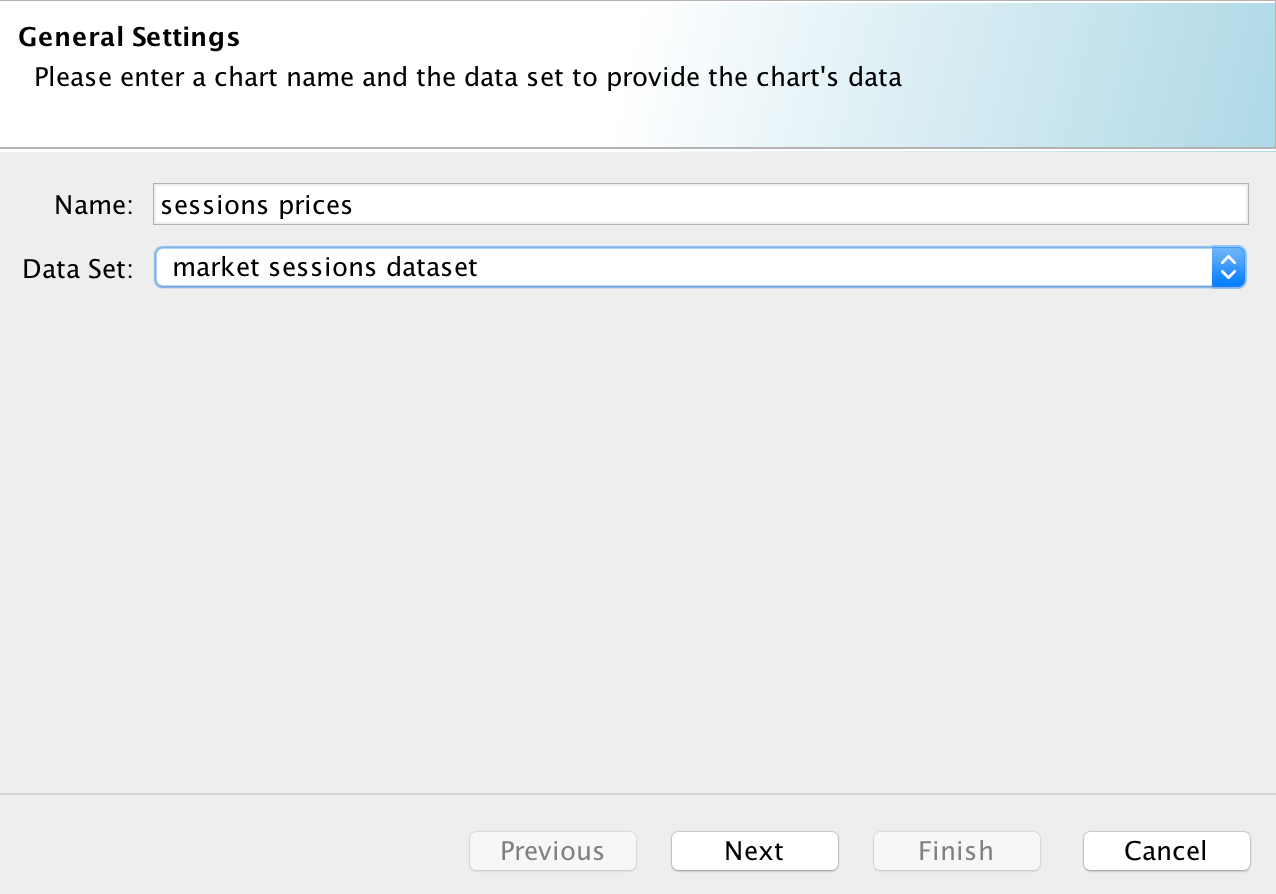
\includegraphics[scale=0.35]{fig_cms_rs_chart1}

A new window appears. The variables in the dataset are displayed. Because we use a Non-Aggregate data set, a legend will be added to identify the lines. The \verb+Series ID+ choice serves to select which variable will be used to this aim. In the following part, the variable to be plotted against time is selected (in this case it is the MarketPrice) 

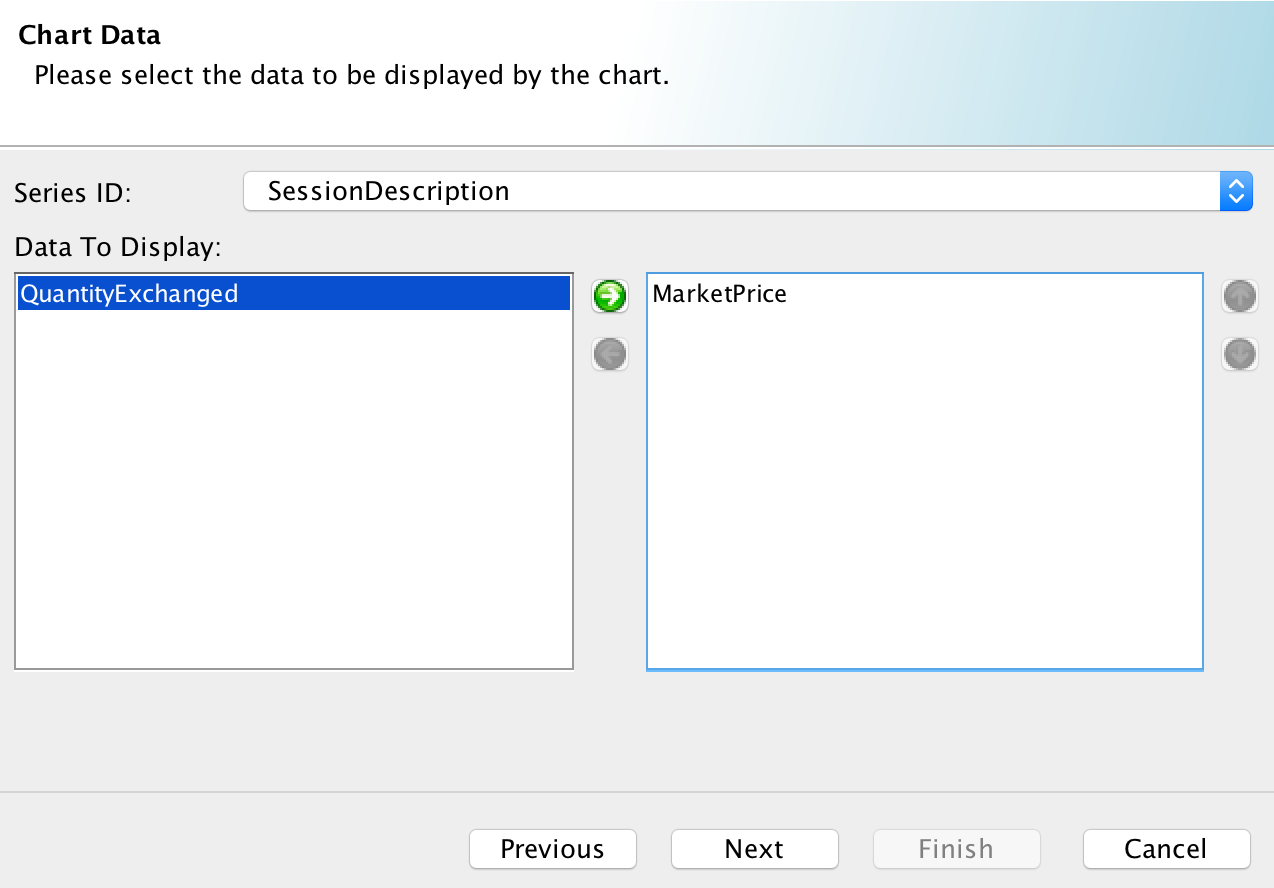
\includegraphics[scale=0.35]{fig_cms_rs_chart2}

The chart titles can be edited in the next wizard window as shown in the figure below

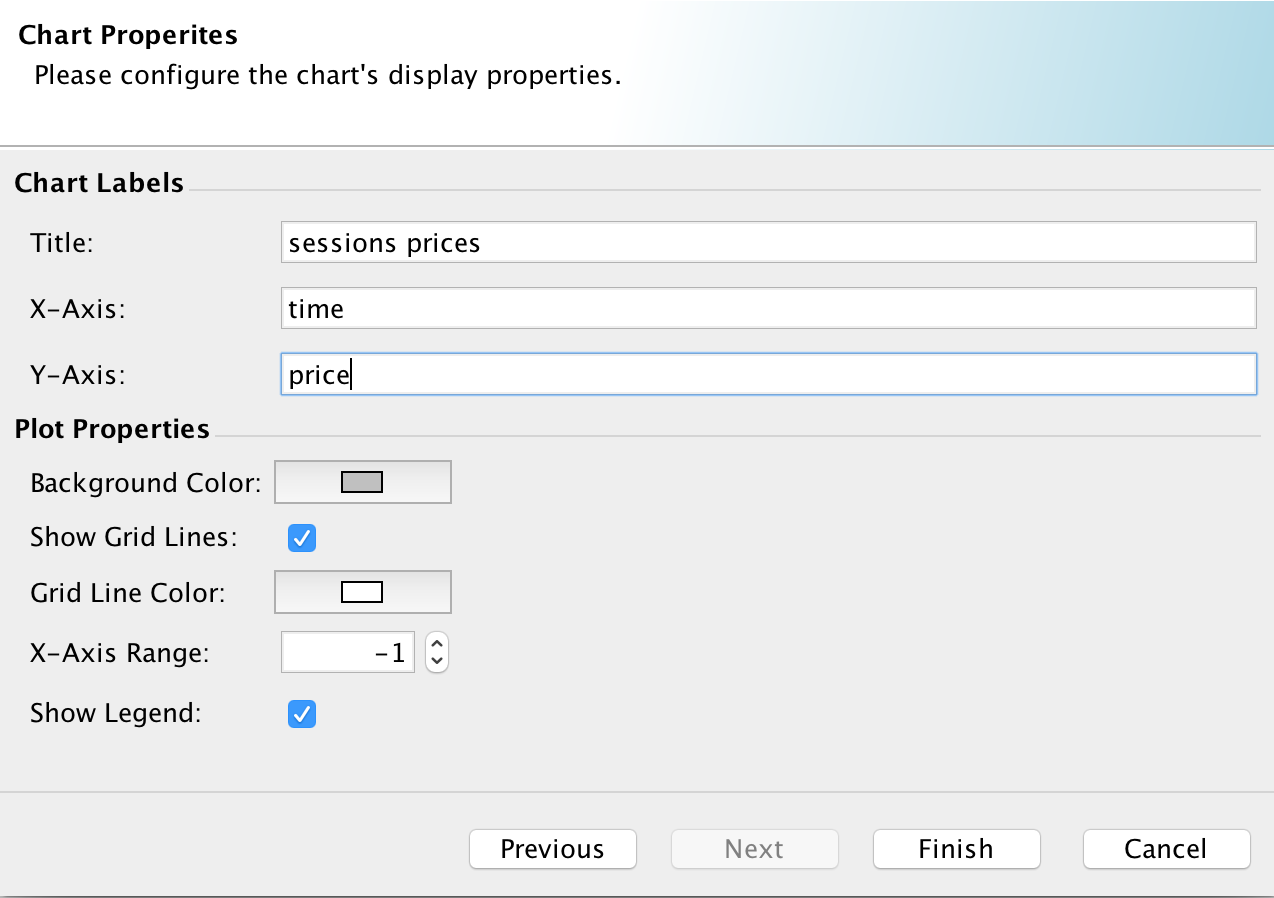
\includegraphics[scale=0.35]{fig_cms_rs_chart3}

Clicking the finish button, the chart item will show up in the Scenario tree as displayed in the next figure

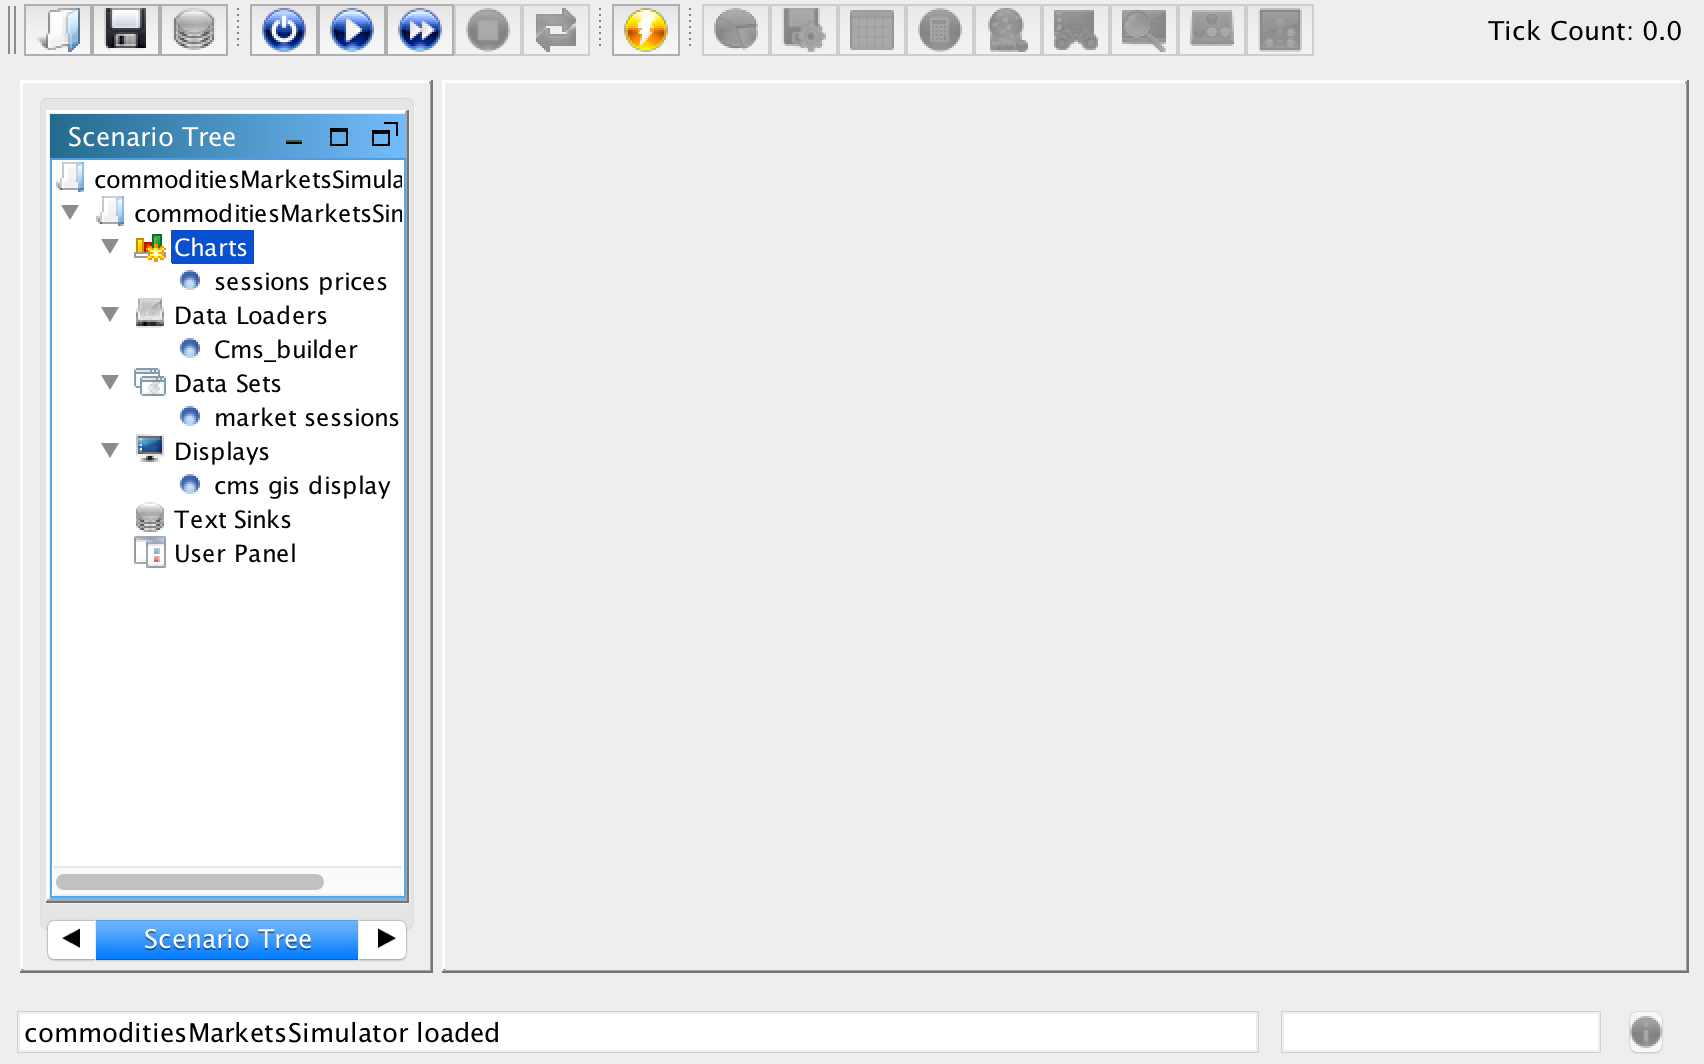
\includegraphics[scale=0.35]{fig_cms_rs_chart4}

By clicking the Step Run button, RS builds all the created graphic elements and lists them in the bar highlighted in the following figure:

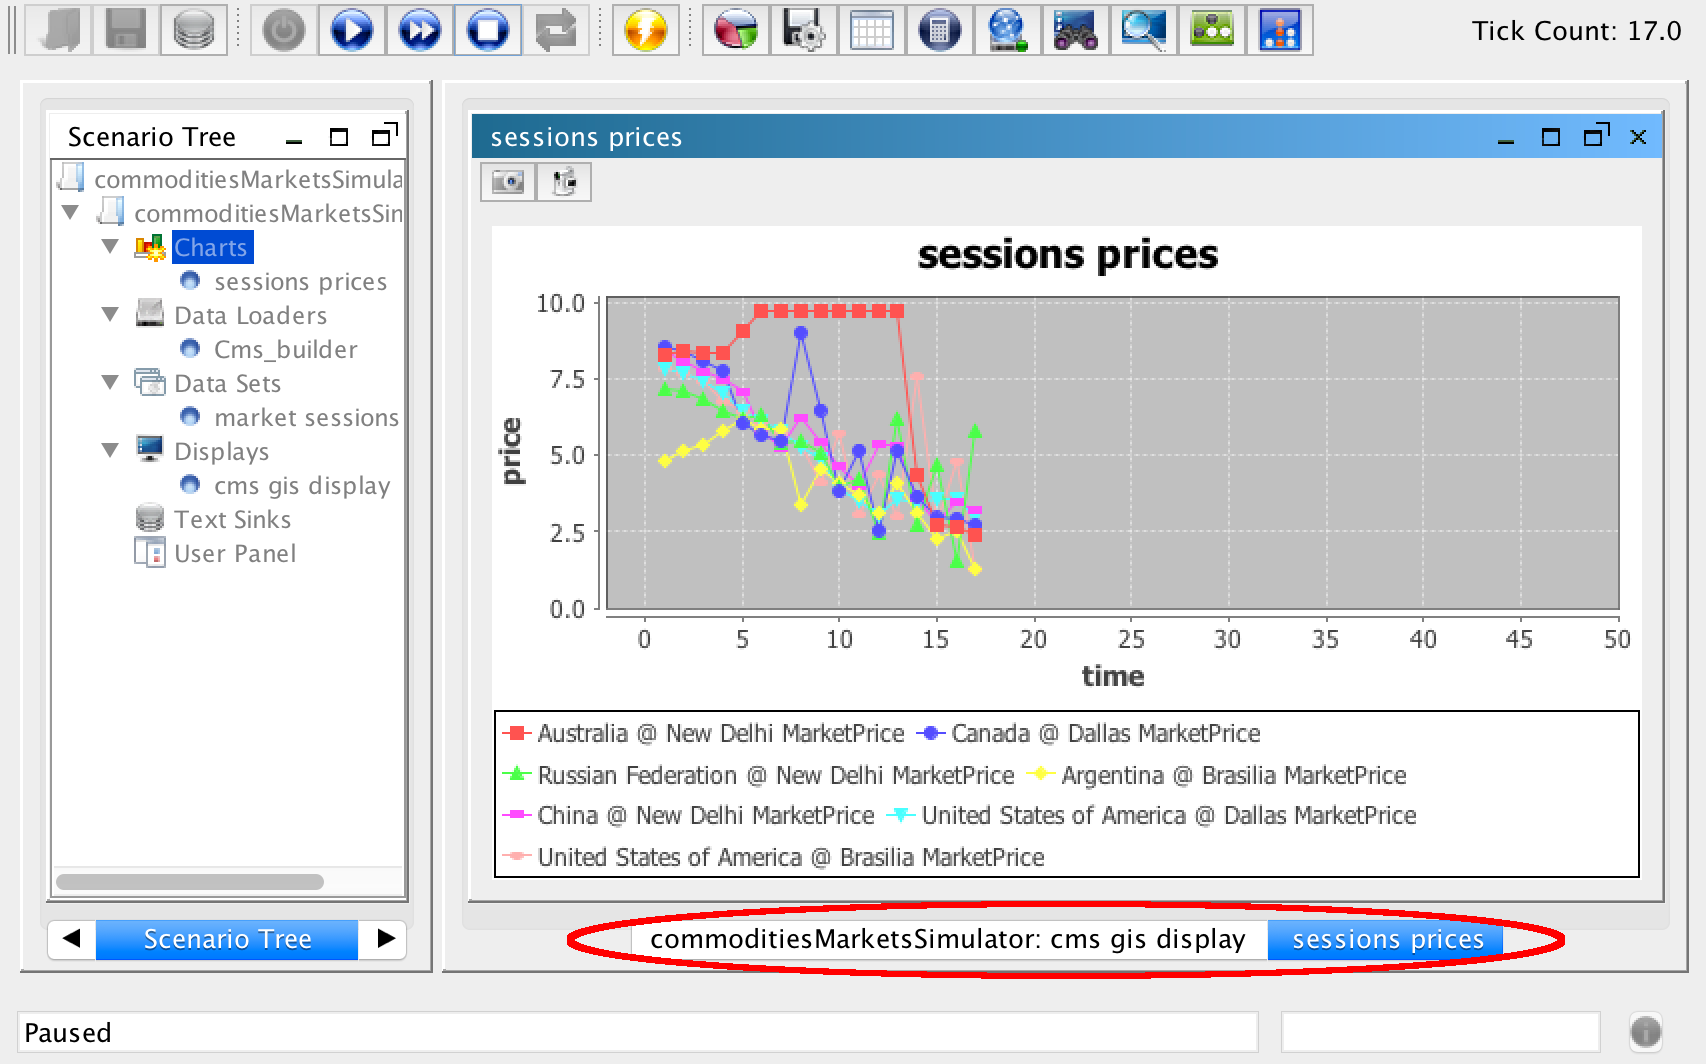
\includegraphics[scale=0.35]{fig_cms_rs_chart5}

It is possible to configure other graphic elements following the process explained above. As an example, using again the \verb+market sessions dataset+ one can build a second chart showing the exchanged quantities. 
Other charts for producers, buyers or aggregate variables can be created provided that data sets for this purpose are previously created. 

Data can be saved by adding \verb+Text Sinks+. The process starts by right clicking the \verb+Text Sinks+ and goes on following the step proposed by the wizard. The reader should be now familiar with this way of creating elements, so we overlook the details pointing readers to the repast data collection documentation. 


\section{Parameter setting}\label{sec:parameters}

There are two types of parameters in this model: aggregate and individual. 

Aggregate parameters relates to the whole economy, therefore they are equal for all the agents. When using the GUI, they can be changed before running the model. To change them, reach the parameters tab in the model GUI by using the arrows highlighted in the following figure.

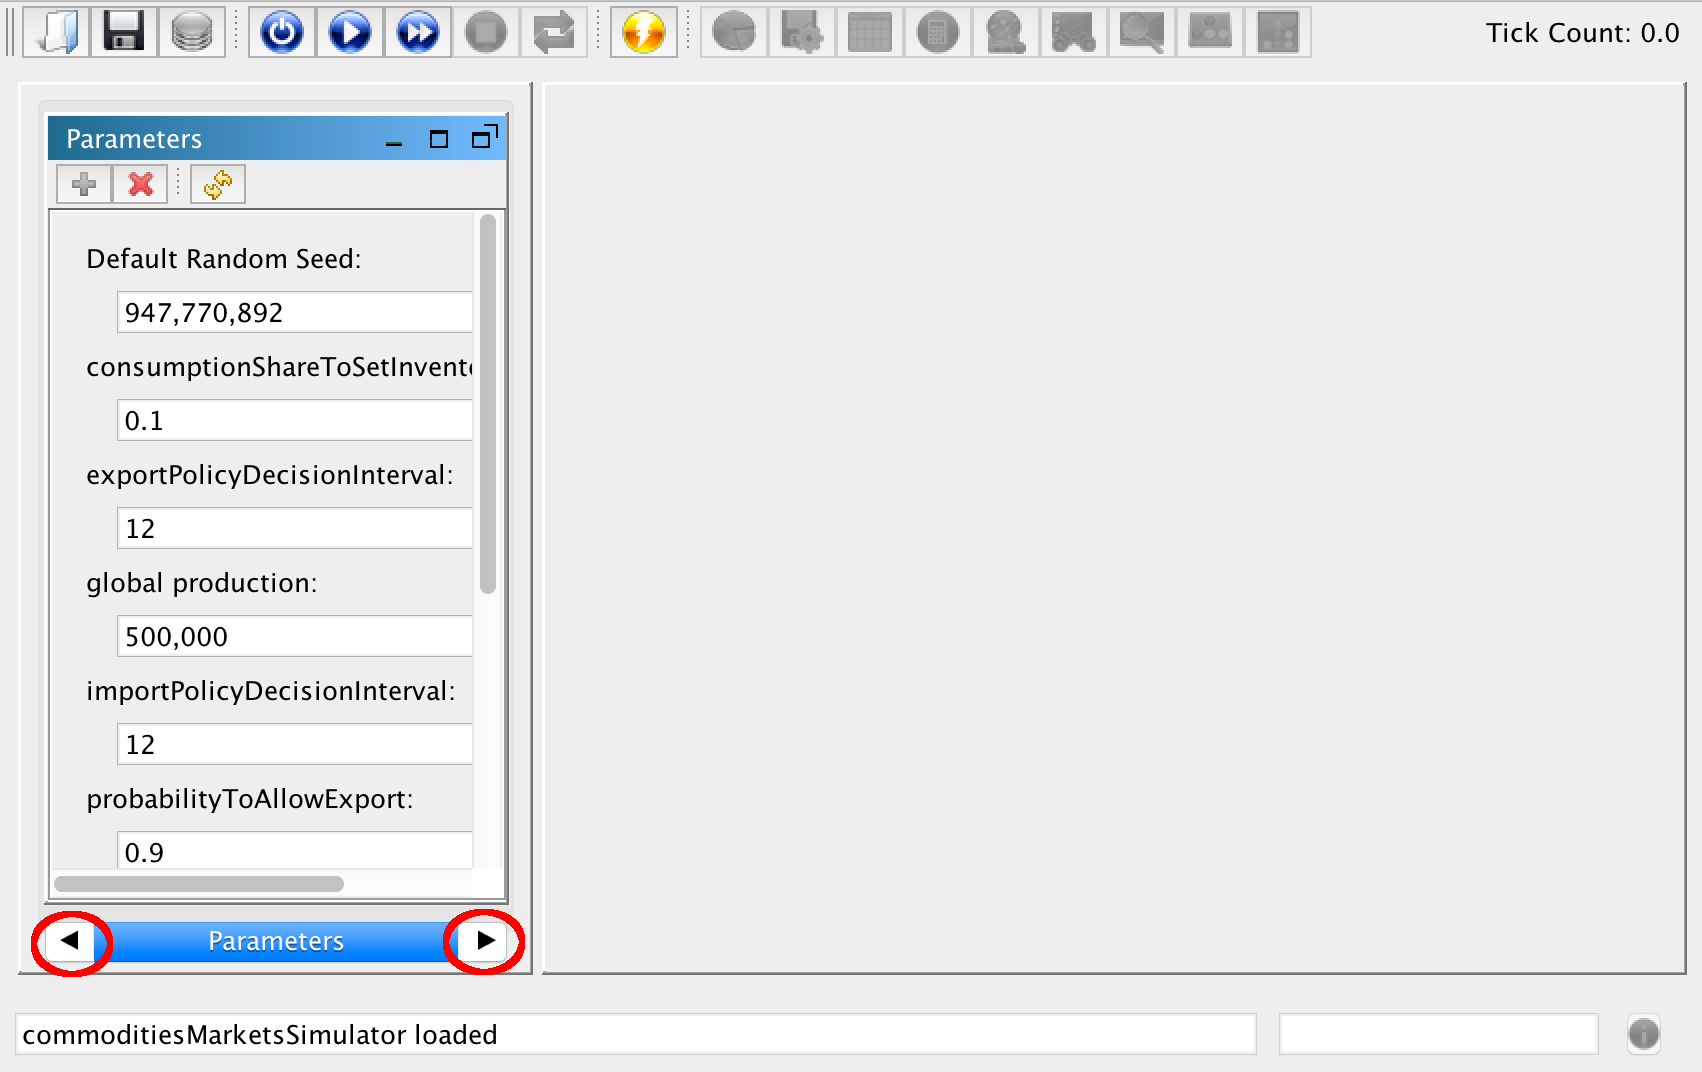
\includegraphics[scale=0.35]{fig_cms_rs_parameters}

Change the parameters and then start running the model. Alternatively, the aggregate parameters can be changed by editing directly the \verb+parameters.xml+ file in the \verb+cms.rs+ folder.


\section{Running in BATCH mode}

To be written

\iffalse
Clicking on the \verb+Batch gabriele model+ as in the following figure

\noindent
%\includegraphics[scale=0.35]{fig_gabriele_rs_execution3}

activates the batch run configuration wizard.

We point the reader to the ``Repast Simphony Batch Runs Getting Started'' document available in RS website for a full description of the wizard.

We only point out that the present version of the model uses custom output recording techniques. Therefore, the RS File Sink are not used. This implies that the ``Optional Output File Patterns'' must be set as in the following figure

\noindent
%\includegraphics[scale=0.35]{fig_gabriele_rs_batch}

This configuration instructs RS to fetch from all the machines running the model in parallel all the file whose name begins with \verb+zdata+  and move them in an output sub-folder named 
\verb+batch_date+. Needless to say that the sub-folder name can be chosen at your convenience, and it can be changed at each batch run in order to avoid overwriting the data (perhaps you want to have memory of the time of your runs. It is why we add \verb+_date+ to the folder name.


The following figure shows the contents of the model output folder after a local batch run using Eclipse navigator panel\\ 
\noindent
%\includegraphics[scale=0.35]{fig_gabriele_rs_batch1}


\fi




\end{document}
